
\chapter{Обобщенное частотное разделение каналов в системе с количеством антенн больше двух}
\section{Модель системы}
В данном разделе мы рассматриваем ОбЧРК МВМВ систему в канале без памяти с Рэлеевским замиранием\cite{Book25}\cite{Book29}. Система может быть описана при помощи выражения \eqref{mim_1} включая в себя канальную и шумовую составляющую в модель. Данная модель не рассматривает многолучевое распространение в среде передачи.
\begin{align}
\mathbf{Y}=\mathbf{HX}+\mathbf{N}
\label{mim_1}
\end{align}
\begin{align*}
\mathbf{H}\in\compl^{M_r\times M_t}
\mathbf{X}\in\compl^{M_t\times T}
\mathbf{N,Y}\in\compl^{M_r\times T}
\end{align*}
 Система ОбЧРК в случае МВМВ так же может быть рассмотрена как модель $PARATUCK2$ третьего порядка. Разница между ОВОВ и МВМВ модели значительна\cite{Book29}, поэтому для использования аналогичной тензорной модели необходимо изменить одну из генерирующих матриц модели, а так же метод формирования двух других. Однако в результате можно описать МВМВ модель при помощи той же тензорной алгебры. Размерность принятых данных равна произведению количества принимающих антенн на размер блока данных.
Матрица символов должна быть составлена из тензора третьего порядка размерности $\mathcal{S}\in \compl^{F\times T_s\times M_t}$ в случае МВМВ модели. Дополнительная размерность связана с тем, что каждая передающая антенна передает свой собственный набор символов не равный с другими антеннами. Однако модель $PARATUCK2$ не предусматривает использование тензоров в модели. Для того чтобы преодолеть данное ограничение тензор $\mathcal{S}$ был переписан как соединенные во второй размерности друг с другом слои по третьей размерности. Выражение можно переписать следующим образом \eqref{mimo_1}. Иначе говоря так же можно сказать что матрица $\mathbf{S}$ равна развертке тензора $\mathcal{S}$ по второй размерности с транспонирование.
\begin{align}
\mathbf{S}=\begin{bmatrix}
\mathcal{S}_{:,:,1}\\
\mathcal{S}_{:,:,2}\\
\vdots \\
\mathcal{S}_{:,:,M_t}\\
\end{bmatrix} \label{mimo_1}
\end{align}
\begin{align*}
\mathcal{S}\in\compl^{F\times T_s\times M_t}
\mathbf{S}\in\compl^{F\cdot M_t\times T_s}
\end{align*}
Матрица$C^{[b]}$ при переходе из ОВОВ модели в МВМВ остается неизменной и не зависит от количества используемых антенн\eqref{mim_2}. В столбцах матрицы остаются фильтрующие последовательность для различных временных слотов которые не зависят от количества антенн. Таким образом правая часть выражения $\mathbf{S}$ не изменяется и имеет аналогичное количество столбцов $T_s$ как в модели ОВОВ.
\begin{align}
\mathbf{C}^{[b]}\in\compl^{T\times T_s}
\label{mim_2}
\end{align}
Вектор связи  $\mathbf{b}$ так же остается не подвергается изменениям при переходе в модель МВМВ \eqref{mimo_3}. Необходимо заметить, что это верно в случае если мы продолжаем рассматривать линейную независящую от времени в пределах передачи одного блока данных модель распространения сигнала. В таком случае вектор  $\mathbf{b}$ будет представлять собой вектор заполненный единичными значениями. 
\begin{align}
\mathbf{b}=\mathbf{1}_{T_s\times 1} \label{mimo_3}
\end{align}
\begin{align*}
\mathbf{b} \in\compl^{T_s\times 1} 
\end{align*}
Матрица $\mathbf{C}^{[a]}$ и $\mathbf{S}$ в случае модели МИМО должны быть изменены. Определим эту матрицу как $\mathbf{C}^{[a]'}$.Согласно размерностям матрицы $\mathbf{S}$, размерность матрицы  $\mathbf{C}^{[a]'}$ должна быть $\mathbf{C}^{[a]'} \in \compl^{T\times F\cdot M_t}$. В сравнении с моделью ОВОВ, в случае МВМВ матрица С должна быть умножена так же с матрицами на основе $\mathbf{C}^{[a]}$. Таким образом матрица $\mathbf{C}^{[a]'}$ должна быть построена на повторении $M_t$ раз матрицы $\mathbf{C}^{[a]}$. Поскольку произведение Адамара представляет собой перенос на другую частоту для каждой из поднесущих модифицированная матрица $\mathbf{C}^{[a]'}$ станет модуляцией всех поднесущих поочередно на каждой из передающих антенн $m_t$. Поскольку все поднесущие на каждой из передающих антенн равны, то их можно собрать простым связыванием одной генерирующей матрицы.
\begin{align}
\mathbf{C}^{[a]'}=
\begin{bmatrix}
\mathbf{C}^{[a]}& \mathbf{C}^{[a]}& \cdots &\mathbf{C}^{[a]}\\
\end{bmatrix} \in\compl^{T\times M_t\cdot F} \label{mimo_4}
\end{align}
\begin{align}
\mathbf{C}^{[a]'}=(\mathbf{1}_{1\times M_t} \otimes \mathbf{C}^{[a]}) \in \compl^{  T\times M_t\cdot F} \label{mimo_5}
\end{align}
Вектор $\amat$ становится  матрицей $\Amat$ и соединяет каждую приемную антенну $m_t$ с каждой поднесущей каждой передающей антенны с коэффициентами передачи для каждой поднесущей.Определим данные коэффициенты в виде тензора $\mathcal{A}$\eqref{mimo_7} включающего коэффициенты для каждой приемной, передающей антенны и поднесущей $m_r,f,m_t$. В модели $PARATUCK2$ тензор $\mathcal{A}$ должен быть представлен в виде матрицы, который будет суммировать все коэффициенты поднесущих  для всех передающих антенн. Размерность матрицы $\Amat$ равна $\Amat \in \compl^{M_r\times F\cdot M_t}$. Таким образом развертка первого порядка тензора $\mathcal{A}$ удовлетворяет данному условию по размерностям\eqref{mimo_8}. 
\begin{align}
\mathcal{A} \in \compl^{M_r\times F\times M_t} \label{mimo_6}
\end{align}
\begin{align}
\mathbf{A}=\mathcal{A}_{[1]} \label{mimo_7}
\end{align}
\begin{align}
\mathbf{A}\in\compl^{M_r \times F\cdot M_t} \label{mimo_8}
\end{align}
Общая модель для МВМВ модели с представленными выше матрицами определена в выражении. Данная модель показывает принятые данные для принятого сигнала без учета влияния шума.Все операции описанные в случае ОВОВ так же могут быть описаны в случае с МВМВ с некоторыми расширениями. Следует заметить что ранг матрицы $\mathbf{A}$ равен $rank(\Amat)=min(M_r,F\cdot M_t)$  и в реальном случае значение в правой части оператора значительно меньше значения в левой его части. Ранг матрицы $\mathbf{A}$  показывает как много потоков передачи данных может открыть система между данным набором антенн. 
\begin{align}
\mathbf{HX}=\mathbf{A}\cdot (\mathbf{C}^{[a]'T} \odot (\mathbf{S}\cdot (\mathbf{C}^{[b]}\diamond \mathbf{B})^T)) \label{mimo_9}
\end{align}
\begin{align*}
\mathbf{HX}\in\compl^{M_r \times T}
\mathbf{A}\in\compl^{M_r \times F\cdot M_t}
\mathbf{C}^{[a]'}\in\compl^{T \times F\cdot M_t}
\end{align*}
\begin{align*}
\mathbf{S}\in\compl^{F\cdot M_t \times T_s}
\mathbf{C}^{[b]}\in\compl^{T \times T_s}
\mathbf{B}\in\compl^{1 \times T_s}
\end{align*}

\section{Ортогонализация влияния канала без частотной избирательности}
Приемник и передатчик совместно могут ортогонализировать влияние канала путем схожим со стандартной ортогонализацией в МВМВ системах. Очевидно подход имеет дополнительные изменения если мы полагаем модель канала равную матрице $\mathbf{A}$. Это связано с тем что ранг матрицы $\mathbf{A}$ значительно меньше количества возможных для ортогонализации потоков. В стандартном подходе для ортогонализации два шага: предобработка и постобработка. Канальная матрица $\mathbf{A}$ может быть разложения при помощи сингулярного разложения матрицы на три матрицы компоненты $\mathbf{U \Sigma V}$.
\begin{align}
\mathbf{A}=\mathbf{U}\cdot \mathbf{\Sigma} \cdot \mathbf{V}^H \label{mimo_co_1}
\end{align}
\begin{align*}
\mathbf{A} \in\compl^{M_r \times F\cdot M_t}
\mathbf{U} \in\compl^{M_r \times M_r }
\mathbf{\Sigma} \in\compl^{M_r \times F\cdot M_t }
\mathbf{V} \in\compl^{F\cdot M_t \times F\cdot M_t }
\end{align*}
\begin{align}
\mathbf{A}=\mathbf{U}_e\cdot \mathbf{\Sigma}_e \cdot \mathbf{V}_e^H \label{mimo_co_2}
\end{align}
\begin{align*}
\mathbf{A} \in\compl^{M_r \times F\cdot M_t}
\mathbf{U} \in\compl^{M_r \times r }
\mathbf{\Sigma} \in\compl^{r \times r }
\mathbf{V} \in\compl^{F\cdot M_t \times r }
\end{align*}
 Передатчик для ортогонализации умножает слева передаваемые данные на матрицу $\mathbf{V}$ которая является матрицей обратной к $\mathbf{V}$. Приемник так же умножает принятые данные на матрицу обратную к матрице $\mathbf{U}$. 
Матрица $\mathbf{\Sigma}$ имеет диагональную структуру и не смешивает данные, однако взвешивает на  коэффициенты. Следует заметить что невозможна диагонализация этим путем количества каналов больше чем ранг матрицы $\mathbf{A}$. Однако как было записано ранее истинное количество потоков данных значительно больше чем ранг $\mathbf{A}$. Стандартный метод не использует ортогональность поднесущих частот и разрушает ортогональную структуру матрицы $\Camat$. Однако структура матрицы $\Camat$ может быть использована для того чтобы ортогонализировать потоки данных соответствующие различным поднесущим у одной и той же передающей антенны. Таким образом строкам в матрице $\mathbf{S}$ могут соответствовать ортогональные из-за различных поднесущих потоки. 
Передатчик обеспечивает предобработку и изменяет матрицу $\Camat$ таким образом чтобы ортогонализировать максимальное количество строк в матрице $\Amat$. Диагонализация в одно частотной МВМВ системе является произведением с матрицей $\mathbf{V}$ из сингулярного разложения матрицы $\mathbf{A}$. Однако а данном случае матрица предобработки будет построена на основе матрицы $\mathbf{V}$ однако будет от нее отличаться. Матрица отрогонализации строится таким образом чтобы тот же базис столбцов соответствовал различным поднесущим одной и той же передающей антенны. Матрица $\mathbf{A}$ состоит из блоков коэффициентов для соответствующей передающей антенны  но разным поднесущим частотам. Согласно ортогональности для различных поднесущих мы можем использовать для тот же самый базис матрицы $\mathbf{V}$. Таким образом приемник получает $r$ параллельных потоков от $M_t$ передающих антенн. Первый блок $M_t$ результирующей $\mathbf{V}_1$ матрицы состоит из повторения одного и того же столбца матрицы $\mathbf{V}$.
\begin{align}
r=rank(\mathbf{A})\label{mimo_co_3}
\end{align}
\begin{align}
\mathbf{V}_1=\begin{bmatrix}\mathbf{V}^{(1)} & \mathbf{V}^{(2)} & \cdots & \mathbf{V}^{(f)} &\cdots&\mathbf{0}^{(r+1)}&\cdots &\mathbf{0}^{(M_t)}\\
\end{bmatrix} \label{mimo_co_4}
\end{align}
\begin{align*}
\mathbf{V}_1\in \compl^{F\cdot M_t \times F\cdot M_t}
\end{align*}
\begin{align}
\mathbf{V}^{(k)}=\begin{bmatrix}
\mathbf{V}_{1,:}^{\mathbf{1}}&\mathbf{V}_{k,:}^{\mathbf{2}}&\cdots &\mathbf{V}_{k,:}^{\mathbf{F}}\\
\end{bmatrix} \in \compl^{F\cdot M_t \times F}
\end{align}
%\begin{align}
%\mathbf{\Sigma}\cdot \mathbf{V}^H \cdot \mathbf{V}_1=[\mathbf{\Sigma}^{(1)}_{1:M_t},\mathbf{\Sigma}^{(2)}_{1:M_t}\cdots \mathbf{\Sigma}^{(F)}_{1:M_t}] \label{mimo_co_5}
%\end{align}
\begin{align}
\mathbf{\Sigma}\cdot \mathbf{V}^H \cdot \mathbf{V}_1=\mathbf{\Sigma}_{1:M_t}\otimes \mathbf{1}_{1\times F} \label{mimo_co_5}
\end{align}
Процесс пост обработки остается аналогичным с классической МВМВ системой. Таким образом пред-обработка и пост-обработка позволяет трансформировать влияние матрицы канала на взвешивание каждого потока данных на какую либо величину при помощи матриц специальной структуры. При этом первые $M_t$ сингулярные значения матрицы $\mathbf{\Sigma}$ умножаются произведение Кронекера с вектором строкой состоящим из единиц. Количество возможных потоков будет зависеть от ранга матрицы $\mathbf{A}$ однако будет сохранять ортогональную структуру матрицы $\Camat$ и увеличивать количество потоков на количество поднесущих.  Общее количество потоков будет равно $rF$. Следует заметить произведение с матрицей обратной с $\mathbf{\Sigma}$ позволит нормализовать потоки данных к одному множителю. Матрица $\mathbf{\Upsilon}$ записана со структурой основанной на произведение Кронекера. Описанная операция позволяет ортогонализировать влияние канала внутри модели $PARATUCK2$. Для ортогонализации передатчик должен лишь домножить с левой стороны передаваемый вектор на сконструированную описанным образом матрицу. Для приемника ортогонализация не будет отличаться от процесса описанного для классической МВМВ ортогонализации.

\begin{align}
\mathbf{\Upsilon}=\mathbf{\Sigma}_e^{-1}\cdot \mathbf{U}^H\cdot \mathbf{U}\mathbf{\Sigma}\cdot \mathbf{V}^H \cdot \mathbf{V}_1=\begin{bmatrix}
\mathbf{1}_{1\times r} \otimes \mathbf{I}_{F}&\mathbf{1}_{1\times (M_t-r)} \otimes \mathbf{0}_{F}\\
\end{bmatrix} \label{mimo_co_6}
\end{align}
\begin{align}
\mathbf{X}=\mathbf{A}\cdot \mathbf{V}_1 (\mathbf{C}^{[a]T} \odot (\mathbf{S}\cdot (\mathbf{C}^{[b]}\diamond \mathbf{B})^T)) \label{mimo_co_8}
\end{align}
\begin{align}
\mathbf{A}^{[o]}=\mathbf{A}\cdot\mathbf{V}_1 \label{mimo_co_9}
\end{align}
\begin{align*}
\mathbf{V}_1 \in\compl^{M_t\cdot F \times M_t\cdot F}
\mathbf{\Delta} \in\compl^{M_r \times M_t\cdot F}
\mathbf{A}^{[o]} \in\compl^{M_r \times M_t\cdot F}
\end{align*}
\section{Поиск коэффициентов передачи поднесущих}
Использование алгоритмов спектрального сканирования так же применимо и в случае с МВМВ моделью. Одно из важных свойств модели МВМВ является разнесенность или свободность зачастую достигаемая при помощи пространственного положения антенн\cite{Book29}. Важно заметить что для различных пар приемник-передатчик может быть занята какая либо поднесущая другой системой. Приемник должен знать матрицу $\mathbf{A}$ для того чтобы знать каким образом были переданы данные. В случае неизвестности для приемника коэффициентов передачи поднесущих задача становится значительно сложнее в силу смешивания данных как во временной так и частотной области. Количество неизвестных для переменных для приемника в таком случае равно $ M_r M_t F$. Количество выражений которые считывает приемник равно для каждого блока данных $TM_r$. Как видно количество неизвестных может быть значительно больше количества известных величин. Однако приемник может найти данные коэффициенты при помощи специальным образом структурированной матрицы символов.
\subsection{Метод поиска основанный на ОВОВ модели}
Одним из способов для поиска матрицы $\mathbf{A}$ является полу-слепой приемник основанный на модели ОВОВ. Приемник может использовать алгоритм описанный в предыдущей части. Передатчик должен сконструировать символы для передачи специальным образом в матрице $\mathbf{S}$ и приемник должен знать как минимум ФМТ символов для поиска всех коэффициентов. Передатчик должен передавать данные как минимум $M_t$ временных слотов с известными символами для того чтобы найти матрицу $\mathbf{A}$. Алгоритм для поиска матрицы $\mathbf{A}$ следующий.
\begin{itemize}
\item Передатчик располагает внутри блока данных специально структурированные символы. Передатчик кладет известные приемнику символы в одну строку для искомой передающей антенны в каждую из поднесущих. Другими словами символы передаются только от определенной передающей антенны каждый временной слот. Передатчик повторяет процесс для каждой передающей антенны в последующие временные интервалы. Таким образом процесс занимает $M_t$ временных интервалов. При этом передатчик должен знать что и когда передавалось.
\item Приемник считывает на входе блок данных с длительностью $M_t$ временных интервалов. Приемник использует полу-слепой алгоритм для ОВОВ и полагает,что принятый сигнал передан от системы с моделью ОВОВ. Таким образом алгоритм позволяет найти значения коэффициентов поднесущих для первой передающей антенны.
\item Приемник повторяет данный процесс $M_t$ раз находя для каждого временного интервала свой блок коэффициентов для того чтобы найти все $M_tM_rF$ коэффициентов матрицы $\mathbf{A}$.
\end{itemize}
\subsection{Алгоритм основанный на МВМВ модели}
Матрица $\mathbf{A}$ может быть найдена при помощи следующего выражения  разделяющего в модели $PARATUCK2$ генерирующую матрицу и векторизированную матрицу $\mathbf{A}$\eqref{mimo_msm_5}. Модель может быть записана как произведение векторизированной матрицы $\mathbf{A}$ и матрицы промежуточной $\mathbf{\Delta}$ являющейся генератором. Данное произведение  может быть выражено с векторизацией для обеих матриц\eqref{mimo_msm_4}. Мы использовали данное свойство для того чтобы найти коэффициенты поднесущих матрицы $\mathbf{A}$ из принятых данных \eqref{mimo_msm_5}. Запишем функцию невязки минимум которой необходимо найти в квадратной норме. При этом выразим невязку относительно векторизированной матрицы $\mathbf{A}$\eqref{mimo_msm_6}. Поскольку функция не является аналитичной изза комплексных значений в матрице $\mathbf{A}$ используем исчисление Виртингера\cite{Book58} для того чтобы найти частную производную по искомому вектору\cite{Book47}. Приравняем производную к нулю и найдем решение полученной системы линейных уравнений. Поскольку оптимизируемая функция является вогнутой, решение у данной системы уравнений будет всего одно и оно будет является точкой минимума.
\begin{align}
\mathbf{Y}=\mathbf{IX}+\mathbf{N} \label{mimo_msm_1}
\end{align}
\begin{align}
\mathbf{X}=\mathbf{A}\cdot (\mathbf{C}^{[a]'T} \odot (\mathbf{S}\cdot (\mathbf{C}^{[b]}\diamond \mathbf{b}^T)^T)) \label{mimo_msm_2}
\end{align}
\begin{align*}
\mathbf{Y,X,N}\in\compl^{M_r\times T}
\end{align*}
\begin{align}
vec(\mathbf{\widehat{X}})=vec(\mathbf{\widehat{A}}\cdot (\mathbf{C}^{[a]'T} \odot (\mathbf{S}\cdot (\mathbf{C}^{[b]}\diamond \mathbf{B})^T))) \label{mimo_msm_3}
\end{align}
\begin{align}
vec(\mathbf{OP})=(\mathbf{P}^T \otimes \mathbf{I})\cdot vec(\mathbf{O}) \label{mimo_msm_4}
\end{align}
\begin{align}
\mathbf{\Delta}=(\mathbf{C}^{[a]'T} \odot (\mathbf{S}\cdot (\mathbf{C}^{[b]}\diamond \mathbf{B})^T)) \label{mimo_msm_5}
\end{align}
\begin{align}
vec(\mathbf{\widehat{X}})=(\mathbf{\Delta}^T\otimes \mathbf{I})\cdot vec(\mathbf{\widehat{A}}) \label{mimo_msm_6}
\end{align}
\begin{align}
\mathbf{r}_5=vec(\mathbf{Y})-vec(\mathbf{\widehat{X}}) \label{mimo_msm_7}
\end{align}
\begin{align*}
\mathbf{\Delta}\in\compl^{M_t\cdot F\times T}
\mathbf{r}_5\in\compl^{M_r\cdot T\times 1}
\end{align*}
\begin{align}
\min_{vec(\mathbf{A})}\mathbf{r}_5^H\mathbf{r}_5 \label{mimo_msm_8}
\end{align}
\begin{align}
\frac{\delta \mathbf{r}_5^H\mathbf{r}_5}{ \delta vec(\mathbf{\widehat{A}}^*)}=0 \label{mimo_msm_9}
\end{align}
\begin{align}
\frac{\delta \mathbf{r}_5^H\mathbf{r}_5}{ \delta vec(\mathbf{\widehat{A}}^*)}=\frac{\delta (vec(\mathbf{Y})-vec(\mathbf{\widehat{X}}))^H(vec(\mathbf{Y})-vec(\mathbf{\widehat{X}}))}{\delta vec(\mathbf{\widehat{A}}^*)}\label{mimo_msm_10}
\end{align}
\begin{align}
\frac{\delta \mathbf{r}_5^H\mathbf{r}_5}{ \delta vec(\mathbf{\widehat{A}}^*)} =(\mathbf{\Delta}^T\otimes \mathbf{I})^H(\mathbf{\Delta}^T\otimes \mathbf{I})vec(\mathbf{\widehat{A}})-(\mathbf{I}\otimes \mathbf{\Delta})^H vec(\mathbf{Y})=0 \label{mimo_msm_11}
\end{align}
\begin{align}
(\mathbf{\Delta}^T\otimes \mathbf{I})^H(\mathbf{\Delta}^T\otimes \mathbf{I})vec(\mathbf{\widehat{A}})=(\mathbf{\Delta}^T\otimes \mathbf{I})^H vec(\mathbf{Y}) \label{mimo_msm_12}
\end{align}
\begin{align}
vec(\mathbf{\widehat{A}})_{opt}=((\mathbf{\Delta}^T\otimes \mathbf{I})^H (\mathbf{\Delta}^T\otimes \mathbf{I}))^{-1}
(\mathbf{\Delta}^T\otimes \mathbf{I})^H vec(\mathbf{Y}) \label{mimo_msm_13}
\end{align}
\begin{align}
vec(\mathbf{\widehat{A}})_{opt}=((\mathbf{\Delta}^*\otimes \mathbf{I}) (\mathbf{\Delta}^T\otimes \mathbf{I}))^{-1}
(\mathbf{\Delta}^*\otimes \mathbf{I}) vec(\mathbf{Y}) \label{mimo_msm_14}
\end{align}
\begin{align}
vec(\mathbf{\widehat{A}})_{opt}=((\mathbf{\Delta}^*\mathbf{\Delta}^T) \otimes \mathbf{I})^{-1}(\mathbf{\Delta}^*\otimes \mathbf{I}) vec(\mathbf{Y}) \label{mimo_msm_15}
\end{align}
\begin{align}
vec(\mathbf{\widehat{A}})_{opt}=((\mathbf{\Delta}^*\mathbf{\Delta}^T)^{-1} \otimes \mathbf{I}^{-1})(\mathbf{\Delta}^*\otimes \mathbf{I}) vec(\mathbf{Y}) \label{mimo_msm_16}
\end{align}
\begin{align}
vec(\mathbf{\widehat{A}})_{opt}=((\mathbf{\Delta}^*\mathbf{\Delta}^T)^{-1}\mathbf{\Delta}^* \otimes \mathbf{I}) vec(\mathbf{Y}) \label{mimo_msm_17}
\end{align}
%\begin{align}
%vec(\mathbf{A})_{opt}= ((\mathbf{I}^H\mathbf{I})\otimes (\mathbf{\Delta}^H\mathbf{\Delta}))^{-1}
%(\mathbf{I}\otimes \mathbf{\Delta})^H vec(\mathbf{Y})
%\end{align}
%\begin{align}
%vec(\mathbf{A})_{opt}= (\mathbf{I}^H\mathbf{I})^{-1}\otimes (\mathbf{\Delta}^H\mathbf{\Delta})^{-1}
%(\mathbf{I}\otimes \mathbf{\Delta})^H vec(\mathbf{Y})
%\end{align}
%\begin{align}
%vec(\mathbf{A})_{opt}= (\mathbf{I}\otimes (\mathbf{\Delta}^H\mathbf{\Delta})^{-1})
%(\mathbf{I}^H\otimes \mathbf{\Delta}^H) vec(\mathbf{Y})
%\end{align}
%\begin{align}
%vec(\mathbf{A})_{opt}= \mathbf{I}\otimes ((\mathbf{\Delta}^H\mathbf{\Delta})^{-1}\mathbf{\Delta}^H) vec(\mathbf{Y})
%\end{align}
Для того чтобы проанализировать ранг искомой обратной матрицы мы проанализировали структуру матрицы. Таким образом можно оценить количество коэффициентов для поиска при помощи одного блока данных. Поскольку ранг произведения Кронекера\eqref{mimo_msm_rank_1} равен произведению рангов исходных матриц рассмотрим входящие в него выражения\eqref{mimo_msm_17}. Единичная матрица имеет максимальный ранг и не является переменной. Таким образом ранг полностью зависит от матрицы $\mathbf{\Delta}$\eqref{mimo_msm_rank_3}. Рассмотрим матрицу $\mathbf{\Delta}$\eqref{mimo_msm_5} , как видно корневая матрица имеет $\mathbf{S} \in \compl^{FM_t\times T_s}$ размеры. Таким образом ранг матрицы $rank(\mathbf{S})= min(FM_t, T_s)$  меньше или равен наименьшей из размерностей. Ранг описанного произведения же $\mathbf{S(C^{[b]}\diamond b^T)^T}$ будет меньше наименьшей из размерностей $rank(\mathbf{S(C^{[b]}\diamond b^T)^T})\leq T_s$. Существует неравенство определяющее ранг произведение Адамара\eqref{mimo_msm_rank_5} и дано в литературе\cite{Book48}\cite{Book56}\cite{Book57}. Поскольку левая часть основана на повторении матрицы $\Camat$ ее ранг следующий $rank(\Camat)= min(FM_t, T_s)$. Тогда ранг произведения будет ограничен следующим верхним порогом. Таким образом мы определили максимальное количество компонент оцениваемых при помощи одного блока данных\eqref{mimo_msm_rank_7}.
\begin{align}
rank(\mathbf{\Delta}^*\mathbf{\Delta}^T)^{-1}\mathbf{\Delta}^*\otimes \mathbf{I}) =(rank(\mathbf{I}))rank((\mathbf{\Delta}^*\mathbf{\Delta}^T)^{-1}\mathbf{\Delta}^*) \label{mimo_msm_rank_1}
\end{align}
\begin{align}
rank(\mathbf{I})=M_r \label{mimo_msm_rank_2}
\end{align}
\begin{align}
rank((\mathbf{\Delta}^*\mathbf{\Delta}^T)^{-1}\mathbf{\Delta}^*)) = rank(\mathbf{\Delta})\label{mimo_msm_rank_3}
\end{align}
\begin{align}
rank(\mathbf{\Delta})\leq rank(\mathbf{C}^{[a]'T})rank((\mathbf{S}\cdot (\mathbf{C}^{[b]}\diamond \mathbf{B})^T)))\label{mimo_msm_rank_4}
\end{align}
\begin{align}
rank(\mathbf{C}^{[a]'T}) =min(T_s,F) \label{mimo_msm_rank_5}
\end{align}
\begin{align}
rank((\mathbf{S}\cdot (\mathbf{C}^{[b]}\diamond \mathbf{B})^T))) = rank(\mathbf{S}) \leq T_s\label{mimo_msm_rank_6}
\end{align}
\begin{align}
rank((\mathbf{\Delta}^H\mathbf{\Delta})^{-1}\mathbf{\Delta}^H)) \leq T_s \cdot min(T_s,F) \label{mimo_msm_rank_7}
\end{align}
\begin{align}
rank(((\mathbf{\Delta}^*\mathbf{\Delta}^T)^{-1}\mathbf{\Delta}^* \otimes \mathbf{I}) ) \leq  T_s\cdot M_t \cdot min(T_s,F)\label{mimo_msm_rank_8}
\end{align}
Передатчик использует данные специальным образом структурированные в матрице символов как объяснено в секции связанной с полу-слепыми приемниками. Тогда мы может найти все коэффициенты при помощи метода наименьших квадратов. В данном случае будут рассмотрены все зависимости в МВМВ модели  и не будет использовано предположений и приближений. Данный подход даст большую точность в определении коэффициентов.
\subsection{Алгоритм основанный на разложении}
Приемник может найти коэффициенты передачи для поднесущих выполнив поиск по меньшему количеству переменных. Это связано с тем что матрица $\mathbf{A}$ в модели $PARATUCK2$ представлена в виде развертки тензора $\mathcal{A}$\cite{}. При этом сам тензор может быть разложен на основополагающие матрицы. При этом размерность неизвестных коэффициентов тензора может быть значительно уменьшена.
\begin{align}
\mathbf{Y}=\mathbf{X}+\mathbf{N}\label{mimo_dsm_1}
\end{align}
\begin{align}
\mathbf{X}=\mathbf{A}\cdot (\mathbf{C}^{[a]'T} \odot (\mathbf{S}\cdot (\mathbf{C}^{[b]}\diamond \mathbf{b}^T)^T))\label{mimo_dsm_2}
\end{align}
\begin{align}
\mathbf{A}=\mathcal{A}_{[1]}=\mathbf{A_A}\cdot(\mathbf{A_C}\diamond \mathbf{A_B})^T\label{mimo_dsm_3}
\end{align}
\begin{align}
\mathbf{X}=\mathbf{A}_A\cdot(\mathbf{A}_C \diamond \mathbf{A}_B)^T \cdot \mathbf{C}^{[a]'T} \odot (\mathbf{S}\cdot (\mathbf{C}^{[b]}\diamond \mathbf{b}^T)^T)) \label{mimo_dsm_4}
\end{align}
\begin{align*}
\mathcal{A} \in \compl^{M_r\times F\times M_t}
\end{align*}
Где $\mathbf{A}_A \in\compl^{M_r\times r} \mathbf{A}_B \in\compl^{F\times r} \mathbf{A}_C \in\compl^{M_t\times r}$ а таким образом приемник может уменьшить количество неизвестных для решения данной задачи\eqref{mimo_dsm_5}. Отношение между $r$ к возможному уменьшению искомых коэффициентов растет полиномиально. Ранг разложения уменьшает количество переменных в случае если ранг разложения будет больше чем заданная величина зависящая от размерностей тензора. Так же существуют дополнительные ограничения для поиска элементов тензора $\mathcal{A}$\eqref{mimo_dsm_7}. 
\begin{align}
N_1=M_r\cdot M_t\cdot F \label{mimo_dsm_5}
\end{align}
\begin{align}
N_2=r\cdot(M_r+ M_t+ F) \label{mimo_dsm_6}
\end{align}
\begin{align}
r=\frac{M_r\cdot M_t\cdot F}{M_r+ M_t+ F} \label{mimo_dsm_7}
\end{align}
\begin{align}
\mathbf{X}=\mathcal{A}_{[1]} \cdot \mathbf{C}^{[a]'T} \odot (\mathbf{S}\cdot (\mathbf{C}^{[b]}\diamond \mathbf{b}^T)^T))\label{mimo_dsm_8}
\end{align}
\begin{align}
\mathbf{X}=\mathbf{A}_A\cdot(\mathbf{A}_C \diamond \mathbf{A}_B)^T  \cdot \mathbf{C}^{[a]'T} \odot (\mathbf{S}\cdot (\mathbf{C}^{[b]}\diamond \mathbf{b}^T)^T))\label{mimo_dsm_9}
\end{align}
\begin{align}
vec(\mathbf{A}_A\cdot(\mathbf{A}_C \diamond \mathbf{A}_B)^T  \cdot \mathbf{C}^{[a]'T} \odot (\mathbf{S}\cdot (\mathbf{C}^{[b]}\diamond \mathbf{b}^T)^T))) \label{mimo_dsm_10}
\end{align}
Запишем выражение в виде векторизированной функции невязки как классическую систему линейных алгебраических уравнений\cite{}. 
\begin{align}
\mathbf{X}=\mathcal{A}_{[1]} \cdot \mathbf{C}^{[a]'T} \odot (\mathbf{S}\cdot (\mathbf{C}^{[b]}\diamond \mathbf{b}^T)^T))\label{mimo_dsm_8}
\end{align}
\begin{align}
\mathbf{X}=\mathbf{A}_A\cdot(\mathbf{A}_C \diamond \mathbf{A}_B)^T  \cdot \mathbf{C}^{[a]'T} \odot (\mathbf{S}\cdot (\mathbf{C}^{[b]}\diamond \mathbf{b}^T)^T))\label{mimo_dsm_9}
\end{align}
\begin{align}
vec(\mathbf{A}_A\cdot(\mathbf{A}_C \diamond \mathbf{A}_B)^T  \cdot \mathbf{C}^{[a]'T} \odot (\mathbf{S}\cdot (\mathbf{C}^{[b]}\diamond \mathbf{b}^T)^T))) \label{mimo_dsm_10}
\end{align}
Возможно разделить операцию векторизации для матрицы $\mathbf{A}_A$ и оставшейся части выражения используя свойства оператора векторизации взятые из источника и записанные в выражении\eqref{mimo_dsm_8}. Таким образом приемник может оценить одну из искомых матриц $\mathbf{A}_A$ с точки зрения наименьших квадратов\eqref{mimo_dsm_15}.
\begin{align}
vec(\mathbf{OP})=(\mathbf{P}^T\otimes \mathbf{I})\cdot vec(\mathbf{O}) \label{mimo_dsm_11}
\end{align}
\begin{align}
vec(\mathbf{X})=vec(\mathbf{A}_A\cdot(\mathbf{A}_C \diamond \mathbf{A}_B)^T  \cdot \mathbf{C}^{[a]'T} \odot (\mathbf{S}\cdot (\mathbf{C}^{[b]}\diamond \mathbf{b}^T)^T))) \label{mimo_dsm_12}
\end{align}
\begin{align}
\mathbf{D}_{in}=(\mathbf{A}_C \diamond \mathbf{A}_B)^T  \cdot \mathbf{C}^{[a]'T} \odot (\mathbf{S}\cdot (\mathbf{C}^{[b]}\diamond \mathbf{b}^T)^T))\label{mimo_dsm_13}
\end{align}
\begin{align}
vec(\mathbf{X})=vec(\mathbf{A_A}  \cdot \mathbf{D}_{in} )\label{mimo_dsm_14}
\end{align}
\begin{align}
vec(\mathbf{X})=(\mathbf{D}_{in}^T\otimes \mathbf{I}_{M_r}) \cdot vec(\mathbf{A_A})\label{mimo_dsm_15}
\end{align}
Приемник может разделить произведение Хатри-Рао на составляющие из выражения  используя другое свойство операции векторизации\eqref{mimo_dsm_c_2}. Таким образом приемник разделяет оставшиеся две матрицы и производит их поиск с точки зрения наименьших квадратов\eqref{mimo_dsm_c_1}. Существует три возможных разделения произведения однако одно из них не выражает необходимым образом искомые матрицы. Поэтому было использовано оставшиеся две формы для того чтобы раскрыть искомые матрицы в необходимом виде.
\begin{align}
vec(\mathbf{OPL})=(\mathbf{L}^T \otimes \mathbf{O}) \cdot vec(\mathbf{P}) \label{mimo_dsm_c_1}
\end{align}
\begin{align}
vec(\mathbf{X})=vec(\mathbf{A}_A\cdot(\mathbf{A}_C \diamond \mathbf{A}_B)^T  \cdot \mathbf{C}^{[a]'T} \odot (\mathbf{S}\cdot (\mathbf{C}^{[b]}\diamond \mathbf{b}^T)^T))) \label{mimo_dsm_c_2}
\end{align}
\begin{align}
vec(\mathbf{X})= ((\mathbf{C}^{[a]'T} \odot (\mathbf{S}\cdot (\mathbf{C}^{[b]}\diamond \mathbf{b}^T)^T))^T \otimes \mathbf{A_A}) vec((\mathbf{A}_C \diamond \mathbf{A}_B)^T)  \label{mimo_dsm_c_3}
\end{align}
\begin{align}
\mathbf{D}_{sec}=((\mathbf{C}^{[a]'T} \odot (\mathbf{S}\cdot (\mathbf{C}^{[b]}\diamond \mathbf{b}^T)^T)) \otimes \mathbf{A_A})\label{mimo_dsm_c_4}
\end{align}
\begin{align}
vec(\mathbf{X})= \mathbf{D}_{sec}\cdot vec((\mathbf{A}_C \diamond \mathbf{A}_B)^T) \label{mimo_dsm_c_5}
\end{align}
\begin{align*}
\mathbf{D}_{in}\in\compl^{T\times M_r\times r}
\mathbf{D}_{sec}\in\compl^{T\cdot M_t\times M_t\cdot F \cdot r}
\end{align*}
Матрицы в произведении Хатри Рао разделяемы выражением даже после транспонирования результата\eqref{mimo_dsm_c_11} \eqref{mimo_dsm_c_12}. Вывод для транспонирования произведения приведен ниже.
\begin{align}
vec((\mathbf{A_C}\diamond \mathbf{A_B})^T)=diag(\mathbf{K}_1\cdot vec(\mathbf{A_C}^T))\cdot \mathbf{K}_2 \cdot vec(\mathbf{A_B}^T) \label{mimo_dsm_c_11}
\end{align}
\begin{align}
\mathbf{L}_B=diag(\mathbf{K}_1\cdot vec(\mathbf{A_C}^T))\cdot \mathbf{K}_2 \in\compl^{M_t\cdot F\cdot r\times F\cdot r } \label{mimo_dsm_c_12}
\end{align}
\begin{align}
vec((\mathbf{A_C}\diamond \mathbf{A_B})^T)= diag(\mathbf{K}_2 \cdot vec(\mathbf{A_B}^T))\mathbf{K}_1\cdot vec(\mathbf{A_C}^T) \label{mimo_dsm_c_13}
\end{align}
\begin{align}
\mathbf{L}_C=diag(\mathbf{K}_2 \cdot vec(\mathbf{A_B}^T))\mathbf{K}_1 \in\compl^{M_t\cdot F\cdot r\times M_t\cdot r } \label{mimo_dsm_c_14}
\end{align}
\begin{align}
\mathbf{K}_1=\begin{bmatrix}
\mathbf{I}_r& \mathbf{0}&\cdots &\mathbf{0}\\
\mathbf{I}_r &\mathbf{0}&\cdots& \mathbf{0}\\
\vdots \\
\mathbf{I}^{F}_r& \mathbf{0}&\cdots &\mathbf{0}\\
\mathbf{0} &\mathbf{I}_r& \cdots& \mathbf{0}\\
\mathbf{0}& \mathbf{I}_r &\cdots& \mathbf{0}\\
&&&\vdots\\
\mathbf{0} &\mathbf{0}&\cdots &\mathbf{I}_r\\
\end{bmatrix}=\mathbf{I}_{M_t}\otimes(\mathbf{1}_{F\times1}\otimes \mathbf{I}_r) \label{mimo_dsm_c_15}
\end{align}
\begin{align}
\mathbf{K}_2=\begin{bmatrix}
\mathbf{I}_{F\cdot r}\\
\mathbf{I}_{F\cdot r}\\
\vdots\\
\mathbf{I}_{F\cdot r}\\
\end{bmatrix} =\mathbf{1}_{M_t\times 1} \otimes \mathbf{I}_{F\cdot r}\label{mimo_dsm_c_16}
\end{align}
В дальнейшем составляется оптимизируемая функция для поиска на основе невязки между принятым и искомым сигналом по отношению ко всем трем матрицам\eqref{mimo_dsm_opt_1}. Мы переписали функцию невязки отдельно для каждого из выражений\eqref{mimo_dsm_opt_3}. Поскольку минимизируемая функция не аналитична м использовали исчисления Виртингера\cite{Book52}\eqref{mimo_dsm_opt_9} для вычисления частным производных по переменным\eqref{mimo_dsm_opt_10}. 
\begin{align}
\min_{\begin{bmatrix}
vec(\mathbf{\widehat{A}_A})\\
vec(\mathbf{\widehat{A}_B})\\
vec(\mathbf{\widehat{A}_C})\\
\end{bmatrix}}(vec(\mathbf{Y})-vec(\mathbf{\widehat{X}}))^H(vec(\mathbf{Y})-vec(\mathbf{\widehat{X}})) \label{mimo_dsm_opt_1}
\end{align}
\begin{align}
\mathbf{r}_4=(vec(\mathbf{Y})-vec(\mathbf{\widehat{X}})) \label{mimo_dsm_opt_2}
\end{align}
\begin{align}
vec(\mathbf{X})=\mathbf{\Gamma}_1 vec(\mathbf{\widehat{A}_A})=\mathbf{\Gamma}_2 vec(\mathbf{\widehat{A}_B}^T)=\mathbf{\Gamma}_3 vec(\mathbf{\widehat{A}_C}^T)\label{mimo_dsm_opt_3}
\end{align}
\begin{align}
\mathbf{\Gamma}_1=(\mathbf{D}_{in}^T \otimes \mathbf{I}_{M_r} ) \label{mimo_dsm_opt_4}
\end{align}
\begin{align}
\mathbf{\Gamma}_2=\mathbf{D}_{sec}\cdot \mathbf{L}_B\label{mimo_dsm_opt_5}
\end{align}
\begin{align}
\mathbf{\Gamma}_3=\mathbf{D}_{sec}\cdot \mathbf{L}_C \label{mimo_dsm_opt_6}
\end{align} 
\begin{align*}
\mathbf{\Gamma}_1\in\compl^{T\cdot M_r\times r \cdot M_r}
\mathbf{\Gamma}_2\in\compl^{T\cdot M_r\times r \cdot F}
\mathbf{\Gamma}_3\in\compl^{T\cdot M_r\times r \cdot  M_t}
\end{align*}
\begin{align}
\mathbf{r}_4=vec(\mathbf{Y})-\mathbf{\Gamma}_1 vec(\mathbf{\widehat{A}_A})=vec(\mathbf{Y})-\mathbf{\Gamma}_2 vec(\mathbf{\widehat{A}_B}^T) \label{mimo_dsm_opt_7}
\end{align}
\begin{align}
\mathbf{r}_4=vec(\mathbf{Y})-\mathbf{\Gamma}_3 vec(\mathbf{\widehat{A}_C}^T)\label{mimo_dsm_opt_8}
\end{align}
\begin{align}
\min_{\begin{bmatrix}
vec(\mathbf{\widehat{A}_A})\\
vec(\mathbf{\widehat{A}_B})\\
vec(\mathbf{\widehat{A}_C})\\
\end{bmatrix}} \mathbf{r}_4^H\mathbf{r}_4 \label{mimo_dsm_opt_9}
\end{align}
\begin{align}
\delta \mathbf{r}_4^H\mathbf{r}_4=\begin{bmatrix}
\frac{\delta \mathbf{r}_4^H\mathbf{r}_4}{\delta vec(\mathbf{\widehat{A}_A}^*)}\\
\frac{\delta \mathbf{r}_4^H\mathbf{r}_4}{\delta vec(\mathbf{\widehat{A}_B}^*)}\\
\frac{\delta \mathbf{r}_4^H\mathbf{r}_4}{\delta vec(\mathbf{\widehat{A}_C}^*)}\\
\end{bmatrix}^T=0 \label{mimo_dsm_opt_10}
\end{align}
\begin{align}
\frac{\delta \mathbf{r}_4^H\mathbf{r}_4}{\delta vec(\mathbf{\widehat{A}_A}^*)}=\frac{\delta (vec(\mathbf{Y})-\mathbf{\Gamma}_1 vec(\mathbf{\widehat{A}_A}))^H(vec(\mathbf{Y})-\mathbf{\Gamma}_1 vec(\mathbf{\widehat{A}_A}))}{\delta vec(\mathbf{\widehat{A}_A}^*)}\label{mimo_dsm_opt_11}
\end{align}
\begin{align}
\frac{\delta \mathbf{r}_4^H\mathbf{r}_4}{\delta vec(\mathbf{\widehat{A}_B}^*)}=\frac{\delta (vec(\mathbf{Y})-\mathbf{\Gamma}_2 vec(\mathbf{\widehat{A}_B}^T))^H(vec(\mathbf{Y})-\mathbf{\Gamma}_2 vec(\mathbf{\widehat{A}_B}^T))}{\delta vec(\mathbf{\widehat{A}_B}^*)}\label{mimo_dsm_opt_12}
\end{align}
\begin{align}
\frac{\delta \mathbf{r}_4^H\mathbf{r}_4}{\delta vec(\mathbf{\widehat{A}_C}^*)}=\frac{\delta (vec(\mathbf{Y})-\mathbf{\Gamma}_3 vec(\mathbf{\widehat{A}_C}^T))^H(vec(\mathbf{Y})-\mathbf{\Gamma}_3 vec(\mathbf{\widehat{A}_C}^T))}{\delta vec(\mathbf{\widehat{A}_C}^*)} \label{mimo_dsm_opt_13}
\end{align}
\begin{align}
\frac{\delta \mathbf{r}_4^H\mathbf{r}_4}{\delta vec(\mathbf{\widehat{A}_A}^*)}= -\mathbf{\Gamma}_1^H(vec(\mathbf{Y})-\mathbf{\Gamma}_1 vec(\mathbf{\widehat{A}_A})) \label{mimo_dsm_opt_14}
\end{align}
\begin{align}
\frac{\delta \mathbf{r}_4^H\mathbf{r}_4}{\delta vec(\mathbf{\widehat{A}_B}^*)}= -\mathbf{\Gamma}_2^H(vec(\mathbf{Y})-\mathbf{\Gamma}_2 vec(\mathbf{\widehat{A}_B}^T))\label{mimo_dsm_opt_15}
\end{align}
\begin{align}
\frac{\delta \mathbf{r}_4^H\mathbf{r}_4}{\delta vec(\mathbf{\widehat{A}_C}^*)}= -\mathbf{\Gamma}_3^H(vec(\mathbf{Y})-\mathbf{\Gamma}_3 vec(\mathbf{\widehat{A}_C}^T)) \label{mimo_dsm_opt_16}
\end{align}
В дальнейшем для минимизации был использован алгоритм ПМНК с последующими шагами:
\begin{itemize}
\item Установка стартовых матриц $\mathbf{\widehat{A}_A,\widehat{A}_B,\widehat{A}_C}$ как случайных комплексных матриц фиксированного размера
\item  Решение СЛАУ $vec(\mathbf{Y})-\mathbf{\Gamma}_1 vec(\mathbf{\widehat{A}_A})$ с данными матрицами  $\mathbf{\widehat{A}_B,\widehat{A}_C}$ и обновлением матрицы $\mathbf{\widehat{A}_A}$ 
\item Решение СЛАУ $vec(\mathbf{Y})-\mathbf{\Gamma}_2 vec(\mathbf{\widehat{A}_B^T})$ с данными матрицами $\mathbf{\widehat{A}_A,\widehat{A}_C}$ и обновлением матрицы  $\mathbf{\widehat{A}_B}$
\item Решение СЛАУ $vec(\mathbf{Y})-\mathbf{\Gamma}_3 vec(\mathbf{\widehat{A}_C^T})$ с данными матрицами $\mathbf{\widehat{A}_A,\widehat{A}_B}$ и обновлением матрицы  $\mathbf{\widehat{A}_C}$
\item Проверка уменьшения значения функции невязки $\frac{\mid\mid vec(\mathbf{Y})-vec(\mathbf{\widehat{X}})\mid\mid^2}{\mid\mid vec(\mathbf{Y})\mid\mid^2}$. В случае если уменьшение больше порога, повторить с алгоритм с пункта 2.
\end{itemize}
Алгоритм ПМНК является очень нестабильным для плохо определенных матриц что делает желаемым использование других методов для поиска точки минимума.
\subsubsection{Анализ ранга вычислений}
Рассмотрим возможный ранг для генерирующих матриц $\mathbf{\Gamma}_1,\mathbf{\Gamma}_2,\mathbf{\Gamma}_3$ для того чтобы понять насколько уменьшится размер исследуемой задачи и количество переменных для оценки. Две генерирующие матрицы состоят из двух частей согласованных с символами и второй частью связанной с разделением произведения Хатри-Рао\cite{Book17}. 
\begin{align}
vec(\mathbf{\widehat{X}})=\mathbf{\Gamma}_1 vec(\mathbf{\widehat{A}_A})=\mathbf{\Gamma}_2 vec(\mathbf{\widehat{A}_B}^T)=\mathbf{\Gamma}_3 vec(\mathbf{\widehat{A}_C}^T)
\end{align}
\begin{align}
\mathbf{\Gamma}_1=(\mathbf{D}_{in}^T \otimes \mathbf{I}_{M_r} ) 
\end{align}

\begin{align}
\mathbf{\Gamma}_3=\mathbf{D}_{sec}\cdot \mathbf{L}_C 
\end{align} 
Рассмотрим матрицу $\mathbf{\Gamma}_1$. Матрица составлена и произведения Кронекера двух других матриц\eqref{ra_1}. Произведение Кронекера имеет ранг соотвествующий выражению\cite{Book19}. При этом единичная матрица имеет полный ранг. Таким образом ранг матрицы полностью зависит от первой части выражения\eqref{ra_2}.
\begin{align}
\mathbf{\Gamma}_1=(\mathbf{D}_{in}^T \otimes \mathbf{I}_{M_r} ) \label{ra_1}
\end{align}
\begin{align}
rank(O\otimes P)=rank(O)rank(P) 
\end{align}
\begin{align}
rank(O\odot P)\leq rank(O)rank(P)
\end{align}
\begin{align}
rank(OP)\leq min(rank(O),rank(P))
\end{align}
\begin{align}
rank(\mathbf{\Gamma}_1)=rank(\mathbf{D}_{in}^T)rank(\mathbf{I}_{M_r}) \label{ra_2}
\end{align}
\begin{align}
\mathbf{D}_{in}^T=(\mathbf{A}_C \diamond \mathbf{A}_B)^T  \cdot \mathbf{C}^{[a]'T} \odot (\mathbf{S}\cdot (\mathbf{C}^{[b]}\diamond \mathbf{B})^T))^T
\end{align}
\begin{align}
rank(\mathbf{C}^{[a]'})=min(F,T)
\end{align}
\begin{align}
rank((\mathbf{C}^{[b]}\diamond \mathbf{b}^T)^T))=min(T_s,T)
\end{align}
\begin{align}
rank{\mathbf{S}} \leq min(F\cdot M_t,T_s)
\end{align}
\begin{align}
rank((\mathbf{S}\cdot (\mathbf{C}^{[b]}\diamond \mathbf{B})^T)) \leq min(F\cdot M_t,T_s,T)
\end{align}
\begin{align}
rank(\mathbf{C}^{[a]'T} \odot (\mathbf{S}\cdot (\mathbf{C}^{[b]}\diamond \mathbf{B})^T)) \leq (min(F\cdot M_t,T_s,T)\cdot min(F,T))\label{ra_3}
\end{align}
\begin{align}
rank(\mathbf{D}_{in}) \leq (min(F\cdot M_t,T_s,T)\cdot min(F,T))\cdot M_r  \label{ra_4}
\end{align}
Верхний порог ранга равен $min(M_t F,T)$\eqref{ra_3} из-за размеров итоговой матрицы. Поскольку $T$ является наибольшей величиной в данном случае, мы можем ей пренебречь и считать что наибольший ранг матрицы известен\eqref{ra_4}.  Реальный ранг не зависит от произведения с рангом матрицы $\Camat $ из-за заполнения матрицы символами.  Рассмотрим произведение Хатри-Рао\cite{Book16}.Результат показан в выражении. Если ранг матрицы полон и равен $T_s$, тогда система ограничена рангом $r$ который позволяет уменьшить ранг матрицы $\mathbf{S}$ от $T_s$ до $r$ для того чтобы найти $\mathbf{A_A}$.
Следующим шагом является анализ матрицы $\mathbf{\Gamma}_2$ и $\mathbf{\Gamma}_3$
\begin{align}
rank(\mathbf{C}^{[a]'T} \odot (\mathbf{S}\cdot (\mathbf{C}^{[b]}\diamond \mathbf{b}^T)^T)) \leq (min(F\cdot M_t,T_s)\cdot F)
\end{align}
\begin{align}
rank(\mathbf{C}^{[a]'T} \odot (\mathbf{S}\cdot (\mathbf{C}^{[b]}\diamond \mathbf{B})^T)) \leq (min(F\cdot M_t,T_s))
\end{align}
\begin{align}
rank((\mathbf{\widehat{A}}_C \diamond \mathbf{\widehat{A}}_B)^T )\leq r
\end{align}
\begin{align}
rank{\mathbf{D}_{in}} \leq min(r,F\cdot M_t,T_s)
\end{align}
Next step is $\mathbf{\Gamma}_2$ rank analysis.
\begin{align}
\mathbf{\Gamma}_2=\mathbf{D}_{sec}\cdot \mathbf{L}_B
\end{align}
\begin{align}
rank(\mathbf{\Gamma}_2)\leq min(rank(\mathbf{D}_{sec}),rank(\mathbf{L}_B))
\end{align}
\begin{align}
\mathbf{D}_{sec}=((\mathbf{C}^{[a]'T} \odot (\mathbf{S}\cdot (\mathbf{C}^{[b]}\diamond \mathbf{B})^T)) \otimes \mathbf{A_A})
\end{align}
\begin{align}
rank(\mathbf{D}_{sec})=rank((\mathbf{C}^{[a]'T} \odot (\mathbf{S}\cdot (\mathbf{C}^{[b]}\diamond \mathbf{b}^T)^T))\cdot rank(\mathbf{\widehat{A}_A})
\end{align}
\begin{align}
rank(\mathbf{\widehat{A}_A})=min(M_r,r)
\end{align}
\begin{align}
rank((\mathbf{C}^{[a]'T} \odot (\mathbf{S}\cdot (\mathbf{C}^{[b]}\diamond \mathbf{b}^T)^T))\leq (min(F\cdot M_t,T_s))
\end{align}
\begin{align}
rank(\mathbf{D}_{sec}\leq (min(F\cdot M_t,T_s))\cdot min(M_r,r)
\end{align}
\begin{align}
\mathbf{L}_B=diag(\mathbf{K}_1\cdot vec(\mathbf{\widehat{A}_C}^T))\cdot \mathbf{K}_2 
\end{align}
\begin{align}
rank(\mathbf{K}_2 )=F\cdot r
\end{align}
\begin{align}
rank(diag(\mathbf{K}_1\cdot vec(\mathbf{\widehat{A}_C}^T)))  \leq (M_t\cdot r)
\end{align}
\begin{align}
rank(\mathbf{L}_B) \leq min((M_t\cdot r),(F\cdot r))
\end{align}
\begin{align}
\mathbf{L}_C=diag(\mathbf{K}_2 \cdot vec(\mathbf{\widehat{A}_B}^T))\mathbf{K}_1 
\end{align}
\begin{align}
rank(\mathbf{K}_1) =r\cdot M_t
\end{align}
\begin{align}
rank(diag(\mathbf{K}_2 \cdot vec(\mathbf{\widehat{A}_B}^T))) \leq F\cdot r
\end{align}
\begin{align}
rank(\mathbf{L}_C) \leq min((M_t\cdot r),(F\cdot r))
\end{align}
\begin{align}
rank(\mathbf{\Gamma}_2)\leq min((M_t\cdot r),(F\cdot r),F\cdot M_t,T_s))\cdot min(M_r,r)
\end{align}
\begin{align}
rank(\mathbf{\Gamma}_3)\leq min((M_t\cdot r),(F\cdot r),F\cdot M_t,T_s))\cdot min(M_r,r)
\end{align}
\section{Полу-слепой приемник для системы с МВМВ}
В предыдущем разделе были рассмотрены решения задачи только для поиска коэффициентов передачи в матрице $\mathbf{A}$. Однако это вносит ограничения в размер передаваемого блока данных и более того не позволяет найти значения переданных символов в случае если они были неизвестны. Таким образом подобные подходы ограничивают размеры передаваемых блоков данных. Для того чтобы увеличить эффективность системы мы можем реализовать полу-слепой приемник определяющий как значения неизвестных символов с матрице $\mathbf{S}$ так и неизвестные коэффициенты канала $\mathbf{A}$. Поскольку мы используем абсолютно ту же модель $PARATUCK2$, алгоритм описанный для ОВОВ модели может быть расширен для модели с МВМВ. В таком случае модулирующие матрицы будут изменены для соответствия модели МВМВ. Так же выражения будут переписаны для векторизации транспонированной матрицы символов $\mathbf{S}$ и матрицы коэффициентов передачи $\mathbf{A}$. Кроме того матрица принятых данных так же будет записана в векторизованной форме после транспонирования $\mathbf{Y^T}$. Так же все остальные выражения не изменяются и остаются прежними. Начальный блок с известными для приемника символами увеличивается от одного до $M_t$ для каждой передающей антенны. Таким образом все оставшиеся символы в блоке данных заполняются символами.
\begin{align*}
\mathbf{r}_1= vec(\mathbf{Y})-\mathbf{\Omega}_1 \cdot vec(\mathbf{S}^T)=\mathbf{r}_2 
\end{align*}
\begin{align*}
\mathbf{r}_2= vec(\mathbf{Y})-\mathbf{\Omega}_2 \cdot vec(\mathbf{A}^T)
\end{align*}
\begin{align*}
\mathbf{r}_3=\mathbf{q} -\mathbf{A}_{sel} vec(\mathbf{S});
\end{align*}
\begin{align}
vec(\mathbf{Y})-\mathbf{\Omega}_1 \cdot vec(\mathbf{S}^T)= vec(\mathbf{Y})-\mathbf{\Omega}_2 \cdot vec(\mathbf{A}^T)
\end{align}
\begin{align}
\mathbf{X}=\mathbf{A}\cdot (\mathbf{C}^{[a]'T} \odot (\mathbf{S}\cdot (\mathbf{C}^{[b]}\diamond \mathbf{B})^T)) 
\end{align}

\begin{align}
\mathbf{\Omega}_1=\begin{bmatrix}
(\mathbf{C}^{[a]'T}\diamond\mathbf{C}^{[b]T}) \diamond (\mathbf{A}_{1,:}\otimes \mathbf{B})\\
(\mathbf{C}^{[a]'T}\diamond\mathbf{C}^{[b]T}) \diamond (\mathbf{A}_{2,:}\otimes \mathbf{B})\\
\vdots\\
(\mathbf{C}^{[a]'T}\diamond\mathbf{C}^{[b]T}) \diamond (\mathbf{A}_{M_r,:}\otimes \mathbf{B})\\
\end{bmatrix}
\end{align}
\begin{align}
\mathbf{\Delta}=(\mathbf{C}^{[a]'T} \odot (\mathbf{S}\cdot (\mathbf{C}^{[b]}\diamond \mathbf{B})^T))
\end{align}
\begin{align}
\mathbf{\Omega}_2=(\mathbf{I}_{M_r}  \otimes \mathbf{\Delta})^T
\end{align}
\begin{align}
\mathbf{J}=\begin{bmatrix}
\frac{\delta \mathbf{r}_1^H\mathbf{r}_1}{\delta vec(\mathbf{S}^*)vec(\mathbf{S})}&\frac{\delta \mathbf{r}_1^H\mathbf{r}_1}{\delta vec(\mathbf{S}^*)vec(\mathbf{A})}\\
\frac{\delta \mathbf{r}_1^H\mathbf{r}_1}{\delta vec(\mathbf{A}^*)vec(\mathbf{S})}&\frac{\delta \mathbf{r}_1^H\mathbf{r}_1}{\delta vec(\mathbf{A}^*)vec(\mathbf{A})}\\
\end{bmatrix}=\begin{bmatrix}
\frac{\delta \mathbf{F}}{\delta vec(\mathbf{S})}&\frac{\delta \mathbf{F}}{\delta vec(\mathbf{A})}
\end{bmatrix} \label{siso_jsm_11}
\end{align}
\begin{align}
\begin{bmatrix}
-\mathbf{\Omega}_1^H(\mathbf{r}_1)+\mathbf{A}_{sel}(\mathbf{r}_3)\\
-\mathbf{\Omega}_2^H(\mathbf{r}_2)\\
\end{bmatrix}=0=\mathbf{F}\label{siso_jsm_12}
\end{align}
\begin{align}
\mathbf{J}=\begin{bmatrix}
\mathbf{\Omega}_1^H\mathbf{\Omega}_1+\mathbf{A}_{sel}&\mathbf{\Omega}_1^H\mathbf{\Omega}_2\\
\mathbf{\Omega}_2^H\mathbf{\Omega}_1&\mathbf{\Omega}_2^H\mathbf{\Omega}_2
\end{bmatrix}\label{siso_jsm_13}
\end{align}
\subsection{Модель системы для канала с памятью}\label{part:SMFSC}
В данном разделе мы рассматриваем модель ОбЧРК с МВМВ в канале с памятью и Рэлеевским замиранием\eqref{m_fsc_1}\cite{Book29}. Укзаанная модель может быть описана в двумя выражениями в матричной и в векторизированной форме. Мы полагаем в системе присутствует защитный интервал между различными блоками данных с длиной не меньшей чем самого большого канала в системе. Таким образом мы можем пренебречь интерференцией между различными блоками данных. Основное выражение системы МВМВ в канале с памятью записывает в следующем виде \eqref{m_fsc_1} согласно источнику\cite{Book53}.
\begin{align}
\mathbf{Y}_{:,k}=\sum^{L}_{l=0}\mathcal{H}_{:,:,l}\mathbf{X}_{:,k-l}+\mathbf{N}_{:,k}
\label{m_fsc_1}
\end{align}
\begin{align*}
\mathbf{Y} \in\compl^{M_r\times T}
\mathbf{N} \in\compl^{M_r\times T}
\mathbf{X} \in\compl^{M_t\times T}
\mathcal{H} \in\compl^{M_r\times M_t \times L+1}
\end{align*}
Где $\mathbf{X}_{:,k}$ выражение соответствует  $k$-тому столбцу переданного блока данных. Размерность каждого столбца равна размерности количества антенн. Тензор $\mathbf{H}$ является тензором третьего порядка, где третьей размерностью являются коэффициенты передачи для различных задержек. При этом запись $\mathbf{H}_{:,:,i}$ полагает $i$-тый слой по третьей размерности из тензора $\mathcal{H}$. Матрица $\mathbf{N}$ является матрицей принятого шума где запись $\mathbf{N}_{:,k}$ полагает $k$-тый столбец от данной матрицы. Мы полагаем что шум является белым Гауссовым шумом без корреляции и с дисперсией $\delta^2$.
Данная модель рассматривает только МВМВ систему не не включает в себя модуляцию данных. Таким образом для описания системы ОбЧРК мы должны включить модулирующую матрицу в описанную модель. Мы можем добавить модулирующую матрицу двумя способами, как переданную матрицу \eqref{m_fsc_2} или в ее векторизированной форме \eqref{m_fsc_3}. Модель переданного сигнала описывается так же как в модели ОбЧРК в канале без памяти однако со специфичной матрицей $\mathbf{A}$. 
\begin{align}
\mathbf{X}=\mathbf{A}\cdot (\mathbf{C}^{[a]'T} \odot (\mathbf{S}\cdot (\mathbf{C}^{[b]}\diamond \mathbf{B})^T)) 
\label{m_fsc_2}
\end{align}
\begin{align}
\mathbf{X}\in\compl^{M_t\times T}
\end{align}
\begin{align}
\mathbf{A}=(\mathbf{I}\otimes \mathbf{1}_{1\times F})\in\compl^{M_t\times M_tF}
\end{align}
\begin{align}
vec(\mathbf{X}^T)=\mathbf{\Upsilon}_1\cdot vec(\mathbf{S}^T)
\label{m_fsc_3}
\end{align}
\begin{align}
\mathbf{\Upsilon}_1=\begin{bmatrix}
(\mathbf{C}^{[a]'T}\diamond\mathbf{C}^{[b]T}) \diamond (\mathbf{A}_{1,:}\otimes \mathbf{B})\\
(\mathbf{C}^{[a]'T}\diamond\mathbf{C}^{[b]T}) \diamond (\mathbf{A}_{2,:}\otimes \mathbf{B})\\
\vdots\\
(\mathbf{C}^{[a]'T}\diamond\mathbf{C}^{[b]T}) \diamond (\mathbf{A}_{M_t,:}\otimes \mathbf{B})\\
\end{bmatrix}
\label{m_fsc_4}
\end{align}
\begin{align}
vec(\mathbf{X}^T)\in\compl^{M_tT\times 1}
\mathbf{\Upsilon}_1 \in\compl^{M_tT\times  FM_tT_s}
vec(\mathbf{S}^T) \in\compl^{FM_tT_s\times  1}
\end{align}
При этом символьная матрица $\mathbf{S}$ абсолютная идентична случаю МВМВ с каналом без памяти и имеет аналогичные размерности $\mathcal{S}\in\compl^{F\times T_s\times M_t}$. Так же следует заметить, что в данном случае мы рассматриваем модель где выполняется условие $T_sF=T$ .
\begin{align}
\mathbf{S}=\begin{bmatrix}
\mathcal{S}_{:,:,1}\\
\mathcal{S}_{:,:,2}\\
\vdots \\
\mathcal{S}_{:,:,M_t}\\
\end{bmatrix} 
\label{m_fsc_5}
\end{align}
\begin{align*}
\mathcal{S}\in\compl^{F\times T_s\times M_t}
\mathbf{S}\in\compl^{F\cdot M_t\times T_s}
\end{align*}
Матрицы $C^{[b]}$,$\mathbf{C}^{[a]'}$ и вектор $\mathbf{b}$ остаются аналогичными в новой модели системы. 
\begin{align*}
\mathbf{C}^{[b]}\in\compl^{T\times T_s}
\end{align*}
\begin{align}
\mathbf{b}=\mathbf{1}_{T_s\times 1} \in\compl^{T_s\times 1} 
\label{m_fsc_7}
\end{align}
\begin{align}
\mathbf{C}^{[a]'}=(\mathbf{1}_{1\times M_t} \otimes \mathbf{C}^{[a]}) \in \compl^{  T\times M_t\cdot F}
\label{m_fsc_8}
\end{align}
Матрица $\mathbf{A}$ имеет специфичную структуру для того чтобы описывать сигнал на выходе передатчика. В изначальном варианте матрица $\mathbf{A}$ указывала связь между приемными и передающими антеннами дял каждой поднесущей. Сейчас же $\mathbf{A}$ указывает на переданный сигнал, следовательно в матрице вместо модели связи между антеннами используется единичная матрица. Тогда матрица $\mathbf{A}$ будет записана следующим образом\eqref{m_fsc_9}.
\begin{align}
\mathbf{A}=\mathbf{I}_{M_t}\otimes \mathbf{1}_{1\times F} \in \compl^{M_t\times F\times M_t} 
\label{m_fsc_9}
\end{align}
Существуют две формы записи канала с памятью, классическая и векторная. Классическая форма \eqref{m_fsc_10} записывается через сумму произведений матриц и не может быть использована для оценки состояния канала. Векторная форма \eqref{m_fsc_11} позволяет записать принятые данные как произведение матрицы на вектор символов как и на вектор канальных элементов. В первом случае матрица будет произведением блочной матрицы свертки со структурой Тоеплитца на матрицу модуляции. Во втором случае матрица будет выражена как матрица свертки относительно переданных данных. Структура матрицы $\mathbf{H}$ представлена на выражении\eqref{m_fsc_12}, где элемент $\mathbf{H_{x,y}}$ является матрицей свертки между $x$-той антенной приемника и $y$-той антенной передатчика\eqref{m_fsc_13}.
\begin{align}
\mathbf{Y}_{:,k}=\sum^{L}_{l=0}\mathcal{H}_{:,:,l}\mathbf{X}_{:,k-l}+\mathbf{N}_{:,k}
\label{m_fsc_10}
\end{align}
\begin{align*}
\mathbf{Y} \in\compl^{M_r\times T}
\mathbf{N} \in\compl^{M_r\times T}
\mathbf{X} \in\compl^{M_t\times T}
\mathcal{H} \in\compl^{M_r\times M_t \times L+1}
\end{align*}
\begin{align}
vec(\mathbf{Y}^T)=\mathbf{H}\cdot \mathbf{\Upsilon}_1\cdot vec(\mathbf{S}^T)=\mathbf{H}vec(\mathbf{X}^T)
\label{m_fsc_11}
\end{align}
\begin{align}
\mathbf{H}=\begin{bmatrix}
\mathbf{H}_{1,1}&\mathbf{H}_{1,2}&\cdots&\mathbf{H}_{1,M_t}\\
\mathbf{H}_{2,1}&\mathbf{H}_{2,2}&\cdots&\mathbf{H}_{2,M_t}\\
\vdots\\
\mathbf{H}_{M_r,1}&\mathbf{H}_{M_r,2}&\cdots&\mathbf{H}_{M_r,M_t}\\
\end{bmatrix}
\label{m_fsc_12}
\end{align}
\begin{align*}
\mathbf{H} \in \compl^{M_r T\times M_t T}
\end{align*}
\begin{align}
\mathbf{H}_{x,y}=\begin{bmatrix}
\mathcal{H}_{x,y,1}&0&0&\cdots&0\\
\mathcal{H}_{x,y,2}&\mathcal{H}_{x,y,1}&0&\cdots&0\\
\mathcal{H}_{x,y,3}&\mathcal{H}_{x,y,2}&\mathcal{H}_{x,y,1}&\cdots&0\\
\vdots\\
\mathcal{H}_{x,y,T}&\mathcal{H}_{x,y,T-1}&\mathcal{H}_{x,y,T-2}&\cdots&\mathcal{H}_{x,y,1}\\
\end{bmatrix}
\label{m_fsc_13}
\end{align}
\begin{align*}
\mathbf{H}_{1,1} \in \compl^{T\times T}
\end{align*}
Мы можем записть векторную форму с выражением вектора канальной матрицы. Для этого мы записываем значения из тензора в следующем порядке\eqref{m_fsc_14}.
\begin{align}
\mathbf{h}=\begin{bmatrix}
vec(\mathcal{H}_{(:,:,1)})\\
vec(\mathcal{H}_{(:,:,2)})\\
\vdots\\
vec(\mathcal{H}_{(:,:,L+1)})\\
\end{bmatrix}
\label{m_fsc_14}
\end{align}
\begin{align*}
\mathbf{h}\in \compl^{(L+1)M_rM_t\times 1}
\end{align*}
Данное выражение позволяет записать векторную форму принятых данных с выделением неизвестного для приемника канала $\mathbf{h}$ в виде векторного произведения. Для этого мы должны определить матрицу векторного произведения$\mathbf{D}_{mod}$. Матрица $\mathbf{D}_{mod}$ записывается в особой форме, составляя матрицу свертки для матрицы переданных, а не вектора как в обычном случае. После чего тензорное произведение с единичной матрицей позволяет увеличить пространство до необходимого количества приемных антенн. Для того чтобы показать процесс в выражении оно было записано поэлементно  \eqref{m_fsc_16}.
\begin{align}
vec(\mathbf{Y})=\mathbf{D}_{mod}\mathbf{h}
\label{m_fsc_15}
\end{align}
\begin{align}
\mathbf{X}=\begin{bmatrix}
x_{1,1}&x_{1,2}&\cdots&x_{1,T}&\\
x_{2,1}&x_{2,2}&\cdots&x_{2,T}&\\
\vdots\\
x_{M_t,1}&x_{M_t,2}&\cdots&x_{M_t,T}&\\
\end{bmatrix}
\end{align}

\begin{align}
\mathbf{D}_{mod}=\begin{bmatrix}
x_{1,1}&\cdots &x_{M_t,1} & 0& \cdots &0&\cdots &0 \\
x_{1,2}&\cdots &x_{M_t,2} &x_{1,1}&\cdots &x_{M_t,1}&\cdots &0 \\
x_{1,3}&\cdots &x_{M_t,3} &x_{1,2}&\cdots &x_{M_t,2}&\cdots &0 \\
\vdots \\
x_{1,T}&\cdots &x_{M_t,T} &x_{1,T-1}&\cdots &x_{M_t,T-1}&\cdots &x_{M_t,1} \\
\end{bmatrix}\otimes \mathbf{I}_{M_r}
\label{m_fsc_16}
\end{align}
\begin{align}
\mathbf{D}_{mod}\in \compl^{TM_r\times (L+1)M_tM_r}
\end{align}
\subsubsection{Метод наименьших квадратов для оценки состояния канала}
Уравнение с выраженным вектором канала позволяет записать оптимизационную задачу для оценки канала при условии что известны все отправленные данные с передатчика. Для этого запишем задачу минимизации второй нормы невязки между принятыми и оцениваемыми данными. Для того чтобы найти оптимальную точку с точки зрения второй нормы невязки \eqref{m_fsc_17} требуется найти частную производную по переменной и найти точку где она будет равна нулю\eqref{m_fsc_18}. Покольку функция является комплексной, она не аналитиичная и от нее нельзя найти производную. Производная может быть найдена при использовании исчисления Виртингера при поиске производной по комплексно сопряженной от переменной $\mathbf{h}^*$. Так как вторая норма невязки является вогнутой функцией, она имеет только одну точку где производная равна нулю и эта точка является искомой \cite{Book54}. Для того чтобы найти эту точку производная должна быть приравнена нулю и найдена точка удовлетворяющая данному условию\eqref{m_fsc_19}. Таким образом решением методом наименьших квадратов будет записано как \eqref{m_fsc_19}.
\begin{align}
\min_{\mathbf{h}}(vec(\mathbf{Y})-\mathbf{D}_{mod}\mathbf{h})^H(vec(\mathbf{Y})-\mathbf{D}_{mod}\mathbf{h})=\min_{\mathbf{h}} \mathbf{r}_m^H\mathbf{r}_m
\label{m_fsc_17}
\end{align}
\begin{align}
\frac{\delta \mathbf{r}_m^H\mathbf{r}_m}{\delta \mathbf{h}^*}=-\mathbf{D}_{mod}(vec(\mathbf{Y})-\mathbf{D}_{mod}\mathbf{h})=0
\label{m_fsc_18}
\end{align}
\begin{align}
\mathbf{h}_{opt}=\mathbf{D}_{mod}^+vec(\mathbf{Y}) 
\label{m_fsc_19}
\end{align}
\subsubsection{Полу-слепой приемник для оценки канала}
Приемник может оценить канал даже в случае если ему неизвестно некоторое количество символов в переданном блоке данных. Для этого  должны строго выполнятся условия определенности задачи и количество неизвестных должно быть меньше количества уравнений. Полу-слепой приемник может быть реализован двумя путями- как ПМНК алгоритм обновляющий постепенно символы и канал либо в алгорите ньютона для одновременного его обновления. Для метода ПМНК требуется записать две функции невязки \eqref{m_ce_1}\eqref{m_ce_2} и на каждой итерации решать задачу для обеих функций. 
\begin{align}
\mathbf{r}_{ms}=vec(\mathbf{Y}^T)-\mathbf{H}\mathbf{\Upsilon}_1vec(\mathbf{S}^T)
\label{m_ce_1}
\end{align}
\begin{align}
\mathbf{r}_{mh}=vec(\mathbf{Y}^T)-\mathbf{D}_{mod}\mathbf{h}
\label{m_ce_2}
\end{align}
Мы рассмотрели три алгоритма дял реализации полу-слепого приемника:: 
\begin{itemize}
\item Приближенный полу-слепой приемник на основе ПМНК
\item Полу-слепой приемник на основе ПМНК с уменьшением собственной интерференции
\item Полу-слепой на алгоритме Ньютона
\end{itemize}
Все три алгоритма описаны ниже. 
\subsubsection{Приближенный полу-слепой приемник на основе ПМНК}
Приближенный полу-слепой приемник конструируется как ПМНК алгоритм в его классической форме. Дополнительная информация от известных символах так же обновляется на каждой итерации, однако игнорируется на этапе обновления переменных. Алгоритм описан пошагово ниже:
\begin{itemize}
\item Задать переменную $\mathbf{S^T}$ как $\mathbf{S^T}_{known}$. Неизвестные символы приравниваются к нулю.
\item Решить СЛАУ \eqref{m_fsc_17} методом МНК \eqref{m_ce_3} и обновить вектор $\mathbf{h}$ .
\item Решить СЛАУ \eqref{m_fsc_17} in the LS sense \eqref{m_ce_4} методом МНК $vec(\mathbf{S}^T)$ и обновить только неизвестные символы.
\item Проверить уменьшение невязки и в случае если она больше порога перейти на шаг 2
\end{itemize}
Выражение для обновления неизвестных показано в \eqref{m_ce_3} и в \eqref{m_ce_4} выражениях ,где $\mathbf{S}_{sel}$  является матрицей выбора где присутсвутют элементы только на диагонали в столбцах неизвестных элементов
\begin{align}
\mathbf{h}_{opt}=\mathbf{D}_{mod}^+vec(\mathbf{Y}) 
\label{m_ce_3}
\end{align}
\begin{align}
vec(\mathbf{S}^T)_{opt}=(\mathbf{I}-\mathbf{S}_{sel})\cdot vec(\mathbf{S}^T_{kn}) \mathbf{S}_{sel}\cdot \mathbf{\Upsilon}_1^+\mathbf{H}^+vec(\mathbf{Y})
\label{m_ce_4} 
\end{align}
\begin{align}
\mathbf{S}_{sel}=\mathbf{I}-diag(vec(\mathbf{S}^T_{known}))^+diag(vec(\mathbf{S}^T_{known})) \in\compl^{M_tFT_s\times M_tFT_s}
\label{m_ce_5}
\end{align}
\subsubsection{Полу-слепой приемник на основе ПМНК с уменьшением собственной интерференции}
Полу-слепой приемник может быть улучшен  при помощи свойства линейности передаваемых данных. В случае если система линейна, известные и неизвестные символы могут быть разделены между собой\eqref{m_ce_6}. Более того модулированные данные так же могут быть разделены на два набора один из которых известен приемнику и второй неизвестный для него. Кроме того матрицы свертки конструируются аналогичным способом. Матрицы выбора позволяют разделить один вектор с известными и неизвестными символами на сумму двух разной или той же размерности
\begin{align}
vec(\mathbf{X}^T)=\mathbf{\Upsilon}_1(vec(\mathbf{S}^T_{kn})+vec(\mathbf{S}^T_{unk}))
\label{m_ce_6}
\end{align}
\begin{align}
vec(\mathbf{X}^T)=\mathbf{\Upsilon}_1vec(\mathbf{S}^T_{kn})+\mathbf{\Upsilon}_1vec(\mathbf{S}^T_{unk})
\label{m_ce_7}
\end{align}
\begin{align}
vec(\mathbf{Y}^T)=\mathbf{H}\mathbf{\Upsilon}_1vec(\mathbf{S}^T_{kn})+\mathbf{H}\mathbf{\Upsilon}_1vec(\mathbf{S}^T_{unk})+vec(\mathbf{E}^T)
\label{m_ce_8}
\end{align}
Приемник не может разделить данные во временной области так как используется модуляция хранящая информацию во всех временных слотах для каждого символа. Однако вычитая из принятого сигнала известную часть мы можем уменьшить собственную интерференцию между символами и увеличить производительность приемника. Таким образом при постановке задачи мы меняем функцию поиска на обновленную \eqref{m_ce_9}.
\begin{align}
\mathbf{r}_{mi}=vec(\mathbf{Y}^T)-\mathbf{H\Upsilon}_1vec(\mathbf{S}^T_{unk})-\mathbf{H\Upsilon}_1vec(\mathbf{S}^T_{kn})
\label{m_ce_9}
\end{align}
\begin{align}
vec(\mathbf{S}^T_{unk})_{opt}=\mathbf{\Upsilon}_1^+\mathbf{H}^+(vec(\mathbf{Y}^T)-\mathbf{H}\mathbf{\Upsilon}_1vec(\mathbf{S}^T_{kn}))
\label{m_ce_10}
\end{align}
\begin{align}
\mathbf{h}_{opt}=\mathbf{D}_{mod}^+vec(\mathbf{Y}) 
\label{m_ce_11}
\end{align}
Обновленные алгоритм для поиска символов и канальной информации записывается следующим образом.
\begin{itemize}
\item Задать переменную $\mathbf{S^T}$ как $\mathbf{S^T}_{kn}$. Неизвестные символы приравниваются к нулю.
\item Решить СЛАУ \eqref{m_ce_9} методом МНК \eqref{m_ce_10} и обновить вектор $\mathbf{h}$ .
\item Решить СЛАУ \eqref{m_ce_9} in the LS sense \eqref{m_ce_11} методом МНК  и обновить $vec(\mathbf{S}^T_{unk})$..
\item Проверить уменьшение невязки и в случае если она больше порога перейти на шаг 2
\end{itemize}
\subsubsection{Регуляризация полу-слепых приемников}
Поскольку задачи по решению обратно задачи свертки являются некорректными, требуется испоьзование дополнительных подходов для увеличения стабильности задачи при работе с шумовой составляющей. Существуют два способа регуляризации при помощи дополнительного члена $\mathbf{V}$ в минимизируемой функции. Они достаточно хорошо описаны в литературе \cite{Book53} и не были использованы в данной работе .
\begin{itemize}
\item Метод подпространств
\item Сглаживание наименьших квадратов.
\end{itemize}  

%\subsubsection{The uncertainty analysis}
%As follows the equation from the previous part, it is not obvious how many symbol should be known for the receiver to estimate the channel and the symbols. The channel and the symbol matrices from \eqref{} and \eqref{} have full rank if at least one symbol is transmitted from each transmit antenna. For that reason dependency from number of the known symbols estimation precision must investigated. 
\subsubsection{Полу-слепой приемник на методе Ньютона}
Полуслепой приемник может использовать оптимизацию основанную на методе Ньютона. Для этого минимизируемая функция должна быть записана в виде системы нелинейных алгебраических выражения и решена в той же форме как и для модели ОВОВ.
 \begin{align}
 \min_{vec(\mathbf{S}_{unk})\mathbf{h}}\mathbf{r}_{mi}^H\mathbf{r}_{mi}
 \label{m_cen_1}
 \end{align}
\begin{align}
\frac{\delta\mathbf{r}_{mi}^H\mathbf{r}_{mi}}{\delta\mathbf{h}^*}=-(\mathbf{D}_u+\mathbf{D}_k)^H(\mathbf{y}-\mathbf{D}_k\mathbf{h}-\mathbf{D}_u\mathbf{h})=0
\label{m_cen_2}
\end{align}
\begin{align}
\frac{\delta\mathbf{r}_s^H\mathbf{r}_s}{\delta vec(\mathbf{S}_{unk})^*}=-(\mathbf{H}\mathbf{\Omega}_k)^H(\mathbf{y}-\mathbf{H}\mathbf{\Omega}_kvec(\mathbf{S}_{kn})-\mathbf{H}\mathbf{\Omega}_uvec(\mathbf{S}_{unk}))=0
\label{m_cen_3}
\end{align}
Минимизируемая функция записывается в следующем виде\eqref{m_cen_1}. Выражение$\mathbf{r}_s$ может быть выписано в двух формах, при этом как и было описан овыше оптимальная точку будет являтся такой точкой \eqref{m_cen_2}, где частная производная по неизвестным будет равна нулю. Такая тояка всего одна в силу того, что минимизируемая функция вогнута. Выпишем частную производную по переменным, используем для этого исчисление Виртингера, так как функция комплексная\eqref{m_cen_3}. Записанное выражение является системой нелинейных уравнений которые требуется решить. Для этого мы используем метод Ньютона как и было сказано выше.

\begin{align}
\mathbf{J}\mathbf{\theta}=-\mathbf{F}
\label{m_cen_4}
\end{align}
\begin{align}
\mathbf{\theta}_{k+1}=\mathbf{\theta}_{k}-\mathbf{J}^+\mathbf{F}
\label{m_cen_5}
\end{align}
\begin{align}
\mathbf{J}=\begin{bmatrix}
\frac{\delta\mathbf{r}_s^H\mathbf{r}_s}{\delta\mathbf{h}^*\mathbf{h}^*}&\frac{\delta\mathbf{r}_s^H\mathbf{r}_s}{\delta vec(\mathbf{S}^*)\mathbf{h}}\\
\frac{\delta\mathbf{r}_s^H\mathbf{r}_s}{\delta\mathbf{h}^*vec(\mathbf{S})}&\frac{\delta\mathbf{r}_s^H\mathbf{r}_s}{\delta vec(\mathbf{S}^*)vec(\mathbf{S})}\\
\end{bmatrix}
\label{m_cen_6}
\end{align}
\begin{align}
\mathbf{F}=\begin{bmatrix}
\frac{\delta\mathbf{r}_s^H\mathbf{r}_s}{\delta\mathbf{h}^*}\\
\frac{\delta\mathbf{r}_s^H\mathbf{r}_s}{\delta vec{\mathbf{S}}^*}
\end{bmatrix}
\label{m_cen_7}
\end{align}
\begin{align}
\mathbf{F}=\begin{bmatrix}
-(\mathbf{D}_u+\mathbf{D}_k)^H(\mathbf{y}-\mathbf{D}_k\mathbf{h}-\mathbf{D}_u\mathbf{h})\\
-(\mathbf{H}\mathbf{\Omega}_k)^H(\mathbf{y}-\mathbf{H}\mathbf{\Omega}_kvec(\mathbf{S}_{kn})-\mathbf{H}\mathbf{\Omega}_u vec(\mathbf{S}_{unk}))
\end{bmatrix}
\label{m_cen_8}
\end{align}
%\begin{align}
%\mathbf{J}=\begin{bmatrix}
%(\mathbf{D}_k+\mathbf{D}_u)^H(\mathbf{D}_k+\mathbf{D}_u) &0\\
%0&(\mathbf{H\Omega}_1)^H\mathbf{H\Omega}_1\\
%\end{bmatrix}
%\end{align}
\begin{align}
\mathbf{J}=\begin{bmatrix}
(\mathbf{D}_k+\mathbf{D}_u)^H(\mathbf{D}_k+\mathbf{D}_u) &(\mathbf{D}_k+\mathbf{D}_u)^H\mathbf{H\Omega}_k \\
(\mathbf{H\Omega}_k)^H(\mathbf{D}_k+\mathbf{D}_u)&(\mathbf{H\Omega}_k)^H\mathbf{H\Omega}_k\\
\end{bmatrix}
\label{m_cen_9}
\end{align}
\begin{align}
\mathbf{\theta}=\begin{bmatrix}
1\\
\mathbf{0}\\
\end{bmatrix}
\label{ce_n_10}
\end{align}
Метод Ньютона решает СЛАУ на каждой итерации для каждой предполагаемой точки решения \cite{Book68}. В качестве модулирующей матрицы для СЛАУ выступает Якобиан для частных производных минимизируемой функции\eqref{m_cen_6}.   Для того чтобы выписать Якобиан мы используем свойство, что минимизируемая функци имеет две одинаковые записи. Таким образом Якобиан записывается следующим образом \eqref{m_cen_9}. К сожалению в данной задаче метод Ньютона является нестабильным и чувствительным к шуму. Для того чтобы уменьшить влияние шума мы использовали простую регуляризацию при помощи суммирования с единичной матрицей до тех пор пока собственное число матрицы не будет меньше порога. Типичное собственное значение Якобина значительно выше 100. Высокое собственное число матрицы приводит к увеличению ошибки. Описание алгоритма Ньютона с использованной регуляризацией описано ниже. Регуляризация позволяет сделать сходимость алгоритма устойчивой и обеспечить сходить даже если матрица очень плохо обусловлена.
\begin{itemize}
\item Установит переменную $\mathbf{\theta}$ следующим образом \eqref{ce_n_10}.
\item Рассчитать Якобиан и частную производную в заданной точке $\mathbf{\theta}$
\item Установить переменную $\lambda=1$.
\item Рассчитать выражение $\mathbf{J}=\mathbf{J+I}\lambda$.
\item  Установить $\lambda=\lambda*2$.
\item Проверить собственное число Якобиана, если оно больше 15, перейти на шаг 4.
\item Решить СЛАУ \eqref{m_cen_4} для переменной $\mathbf{\theta}$
\item Обновить переменную $\mathbf{\theta}$ при помощи выражения \eqref{m_cen_5} .
\item Если невязка уменьшилась на значение больше порогового, перейти на шаг 2.
\end{itemize}

\section{Результаты моделирования}
В данной секции представлены результаты моделирования ОбЧРК системы с МВМВ моделью и показаны результаты работы алгоритмов представленных выше.
\begin{table}[H]
\caption{\label{tab:sim_alpha}ОбЧРК эксперимент 2.1}
\begin{center}
\begin{tabular}{|c|c|c|}
\hline
Параметр & Обозначение & Значение \\
\hline
\hline
Схема модуляци & $\mu$ & КФМ-2 \\
\hline
Отсчетов на символ & $T/T_s$ & 16 \\
\hline
Поднесущих&$F$&16 \\
\hline
Размер блока данных& $T_s$  &5 \\
\hline
Вид фильтра&  &КиПК \\
\hline
Коэффициент перекрытия&$\alpha$  &0.5 \\
\hline
Коэффициенты поднесущих& $\mathbf{a}_i$ & $randi([0 1])$ \\
\hline
Канал& $h$ &АБГШ \\
\hline
Префикс&  & Нет \\
\hline
Передача&  & Некодированная \\
\hline
\end{tabular}
\end{center}
\end{table}
\begin{figure}[H]
\centering
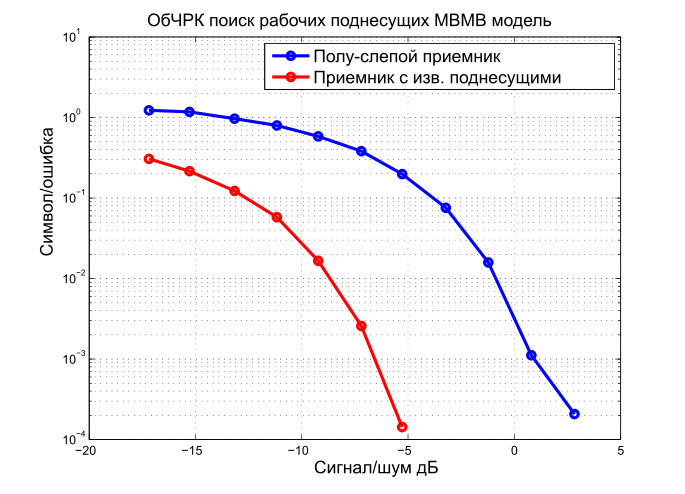
\includegraphics[width=0.9\columnwidth]{MIMO_SER_1.png}
\caption{\label{fig:fs_m_1}\textit{Производительность работы алгоритма поиска поднесущих для случая МВМВ}}
\end{figure}
\begin{figure}[H]
\centering
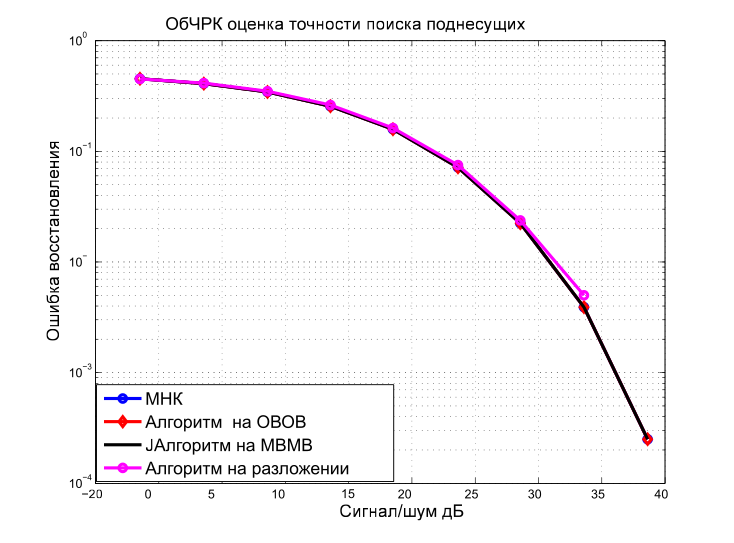
\includegraphics[width=0.9\columnwidth]{SM_RE_MIMO.png}
\caption{\label{fig:fs_m_2}\textit{Ошибка восстановления поднесущих для алгоритма поиска поднесущих для случая МВМВ}}
\end{figure}
Производительность системы ОбЧРК для работы алгоритма ортогонализации получены при помощи моделирования. В системе был положен аддитивный белый Гауссов шум без какого либо кодирования. В системе была использована квадратурная фазовая манипуляция. Количество поднесущих равно $F=16$. Количество временных отсчетов на каждый временной символ равно $T/T_s=F$. Количество временных символов равно $T_s=5$. В качестве фильтра был использован фильтр с характеристикой "Корень из приподнятого косинуса" с коэффициентом перекрытия $\alpha=0.5$. Коэффициенты канальной матрицы $\Amat$ были выбраны как случайные комплексные величины с нулевым моментом первого порядка и среднеквадратичным отклонением модуля числа равным $1$. В системе был использован приемник на основе псевдообратной матрицы. На первом  рисунке представлены результаты работы алгоритма по ортогонализации влияния канала. Мы сравнивали подход с МВМВ канальной ортогонализацией. Результаты показаны на  рис. для приемника на основе псевдообратной матрицы.
\begin{figure}[H]
\centering
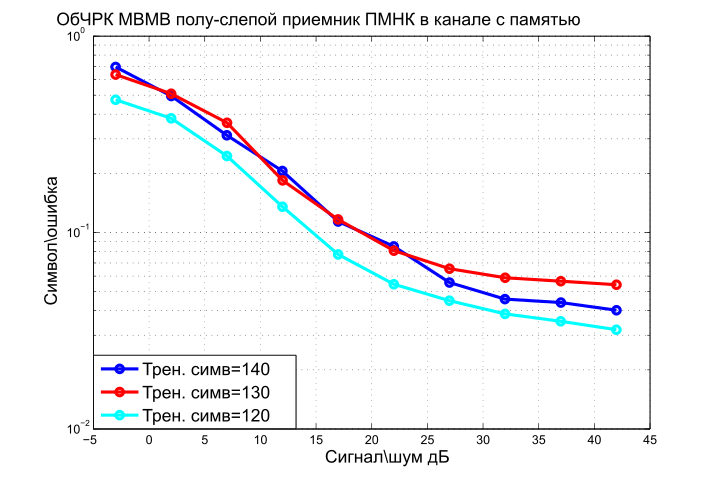
\includegraphics[width=0.9\columnwidth]{SM_MIMO_SER_ALS.png}
\caption{\textit{Производительность работы полу-слепого приемника для канала с памятью и системы МВМВ}}
\label{fig:fs_m_3}
\end{figure}
\begin{figure}[H]
\centering
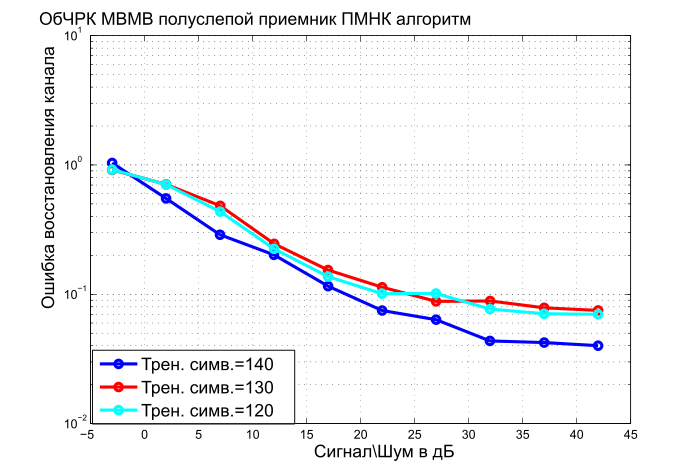
\includegraphics[width=0.9\columnwidth]{SM_MIMO_RE_ALS.png}
\caption{\textit{Ошибка восстановления канала полу-слепого приемника для канала с памятью и системы МВМВ}}
\label{fig:fs_m_4}
\end{figure}
Производительность системы ОбЧРК для сравнения поиска величин $\Amat$ коэффициентов получены при помощи моделирования. В системе был положен аддитивный белый Гауссов шум без какого либо кодирования. В системе была использована квадратурная фазовая манипуляция. Количество поднесущих равно $F=16$. Количество временных отсчетов на каждый временной символ равно $T/T_s=F$. Количество временных символов равно $T_s=5$. В качестве фильтра был использован фильтр с характеристикой "Корень из приподнятого косинуса" с коэффициентом перекрытия $\alpha=0.5$. Коэффициенты канальной матрицы $\Amat$ были выбраны как случайные целочисленные величины с возможными значениями равными 0 и 1. Результаты работы ОбЧРК представлены на двух рисунках, на первом показаны соотношения символов к количеству ошибок. Для сравнения так же показаны варианты когда система знает истинные коэффициенты матрицы $\mathbf{A}$ и находит решение на основе псевдообратной матрицы. На втором показана ошибка определения значения матрицы $\mathbf{A}$ нормализованное к истинной величине.
\begin{table}[H]
\caption{\label{tab:m_table3}ОбЧРК эксперимент 2.2}
\begin{center}
\begin{tabular}{|c|c|c|}
\hline
Параметр & Обозначение & Значение \\
\hline
\hline
Передающие антенны кол-во &$M_t$&2 \\
\hline
Приемные антенны кол-во  &$M_r$&2 \\
\hline
Схема модуляции & $\mu$ & 2(КФМ) \\
\hline
Отсчетов на символ & $T/T_s$ & 16 \\
\hline
Поднесущие &$F$&16 \\
\hline
Размер блока& $T_s$  &5 \\
\hline
Вид фильтра&  &КиПК \\
\hline
Коэффициент перекрытия&$\alpha$  &0.5 \\
\hline
Коэффициенты поднесущих & $\mathbf{a}_i$ & $randi([0 1])$ \\
\hline
Канал& $h$ &АБГШ \\
\hline
Префикс&  & Нет \\
\hline
Передача&  & Некодированная \\
\hline
Ранг разложения& $rank$ & 25\\
\hline
\end{tabular}
\end{center}
\end{table}
\begin{figure}[H]
\centering
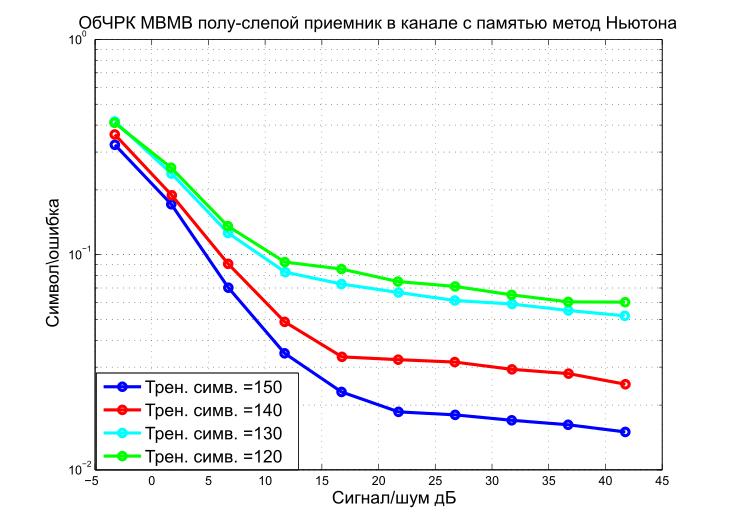
\includegraphics[width=0.9\columnwidth]{SM_MIMO_SER_N.png}
\caption{\textit{Производительность работы полу-слепого приемника для канала с памятью и системы МВМВ. Метод Ньютона}}
\label{fig:fs_m_5}
\end{figure}
\begin{figure}[H]
\centering
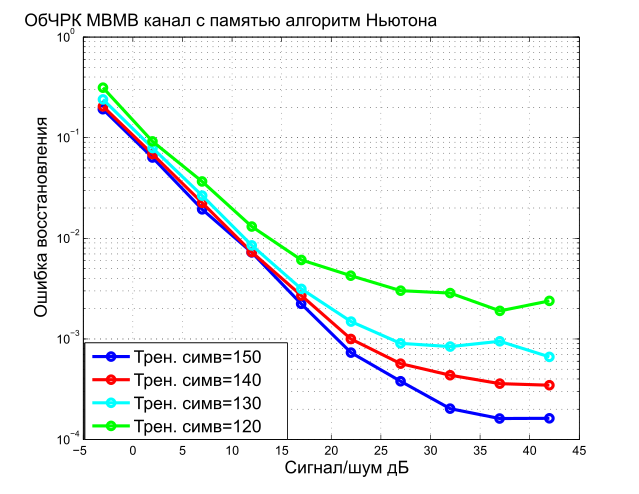
\includegraphics[width=0.9\columnwidth]{SM_MIMO_RE_N.png}
\caption{\textit{Ошибка восстановления канала полу-слепого приемника для канала с памятью и системы МВМВ. Метод Ньютона}}
\label{fig:fs_m_6}
\end{figure}
Полу-слепой приемник дял оценки канала и неизвестных символов основанный на методе Ньютона в системе МВМВ был оценен по производительности при помощи симуляции. Для симуляции была использована квадратурная фазовая модуляция. Канал был создан в два этапа: в качестве канала с памятью был использован канал $Ped-A$ из стандартов IEEE, в качестве модели различных антенн было использовано Рэлеевское замирание в канале. Для этого генерировалась матрица случайных комплексных величин $\mathcal{H}$ с дисперсией равной единице. После этого использовалось произведение по третьему пространству для получения канального тензора$\mathcal{H}$. Количество приемных и передающих антенн задано изначально $M_r=M_t=2$. Количество поднесущих было $F=16$, временных отсчетов на символ $T/T_s=F$. Размер блока был задан $T_s=5$. В качестве фильтра был использован корень из Приподнятого косинуса с коэффициентом перекрытия $\alpha=1$. Длина канала вычислялсь исходя из модели  и имела фиксированную длительность $L+1=4$. Параметры эксперимента так же представлены в табл.\ref{tab:m_table3}. Результаты производительности ОбЧРК показаны на двух графиках. На рис. \eqref{fig:fs_m_5} представлена производительность системы по распознаванию символов. Эксперимент показывает зависимость количества тренировочных символов в блоке и соотношения сигнал/шум. На рис.  \eqref{fig:fs_m_6} показана ошибка восстановления канала от аналогичных переменных.
Выражение для ошибка восстановления указано в \eqref{sim:eq_m_2}.
\begin{align}
R_e=\frac{\mid\mid\mathbf{h-\widehat{h}}\mid\mid^2}{\mid\mid\mathbf{h}\mid\mid^@}
\label{sim:eq_m_2}
\end{align}

\section{Заключение}
В первом эксперименте был исследован алгоритм поиска рабочих поднесущих в системе ОбЧРК с случае МВМВ. Как мы видим из результатов эксперимента, производительность по сравнению с эталоном для которого известны поднесущие упала на 5-6 дБ с точки зрения соотношения символы/ошибки. Данные результат виден из рис. \ref{fig:fs_m_2}. Падение в производительности связано с тем что в алгоритме был использован очень простой метод принятия решения по определению включенных поднесущих. Поскольку данная задача является задачей классификации, а мы используем регрессионный метод для поиска значений в алгоритме было использовано простейшее решающее устройство на основе порога. В случае если порог был меньше чем абсолютное значение оцениваемого коэффициента, поднесуащя считалась включенной. Таким образом используя более точные методы принятия решени можно добиться лучшего результата.

В качестве алгоритмов оценки поднесущих мы описали 3 различных алгоритма каждый из который действует различным методом, однако как показали результаты все они показывают одинаковую точность при принятии решений, что видно из рис.\ref{fig:fs_m_3} .Даже приближенный метод оценки позволяет оценить поднесущие с абсолютно той же точностью. Это может быть связано с тем, что решающее устройство на всех алгоритмах было одинаково, либо ошибка приближенного метода является несущественной. Однако следует отметить, что метод основанный на разложении чувствителен к выбору начальной точки, что делает сходимость алгоритма нестабильной. Из-за этого в результаты в графиках представлены в медианной оценке. Однако как можно видеть по медианной оценке, это не влияет на статистическую сходимость алгоритма.

Как видно из второго эксперимента полу-слепой приемник на основе алгоритмов ПМНК позволяет получать как символы так и оценивать состояние канала. Точность оценки к сожалению не высокая, что связано с достаточно сложными условиями приема, когда проявляется нестабильность соединения между антеннами, и проявления памяти канала для каждого из соединений. Как видно из рис.  \ref{fig:fs_m_3}, количество ошибок в системе ограничено снизу и производительность не оказывается лучше постоянного коэффициента. Более того аналогичный результат виден и в случае оценки состояния канала на рис. \ref{fig:fs_m_4}. Это связано с плохой обусловленностью системы. Кроме того состояние канала и коэффициенты связи между антеннами могут вместе получать эффект значительного ухудшения собственного числа матрицы канала. Таким образом как заключение к алгоритму можно сказать о необходимости использования регуляризующих коэффициентов. Поскольку задача является некорректно поставленной по Тихонову, можно использовать различные алгоритмы стабилизации решения у точки минимума. Однако можно сказать, что сама система имеет значительны потенциал и может показывать значительно лучшие результаты. Так же следует рассмотреть реальные модели канала МВМВ с памятью и типичные модели работы данного канала. Данные модели будут рассмотрены в дальнейшей работы.

Следующий эксперимент показывает производительность полу-слепого приемника на методе Ньютона. Канала вд данной модели полагается каналом с памятью модели $Ped-A$ взятый из стандарта IEEE умноженный по третьему пространству с матрицей случайных элементов с дисперсией равной единице. На рис. показана производительность алгоритма по распознаванию символов. Как видно из графика производительность алгоритма так же ограничена сверху и очень сильно зависит от количества тренировочных символов. Это связано с тем, что в относительном измерении количество канальных переменных велико. При этом от собственное число матрицы канала чрезвычайно велико и приводит к значительным погрешностям при работе алгоритма. Для устранения подобного влияния необходимо использование дополнительных методов как и было описано в предыдущем эксперимента. Однако в данном случае эти методы должны быть внедрены чрезвычайно аккуратно, так как метод второго порядка и очень чувствителен к возможным методам регуляризации.
Как видно из рис. точность определения канала значительно выше, чем символов и зависит в меньшей степени от количества символов. Количество тренировочных символов сказывается лишь на верхнем лимите. Данный эффект проявляется только при высоком соотношении сигнал/шум. В дальнейшей работе будут рассмотрены дополнительные алгоритмы по регуляризации и увеличению точности работы полу-слепого приемника а так же модели канала существующие в МВМВ системах. В качестве основных тезисов по работе полу-слепого приемника можно выделить следующее:
\begin{itemize}
\item Производительность приемника по распознаванию символов мала
\item Производительность приемника по оценке канала применима для работы в алгоритмах
\item Требуется использование регуляризирующих алгоритмов
\end{itemize}



%The last experiment show performance of the Newton based semi-blind receiver over the frequency selective Rayleigh fading channel. The fig.\eqref{fig:fs_m_5} show the performance of the algorithm in the symbol estimation. As we can see here the algorithm has the upper bound in the performance and doesn't allow to decrease the SER lower than $10^{-2}$. This behavior doesn't connected with error in the channel estimation, because the error in the channel estimation is upper bounded with much higher SNR and have precision near to the $10^{-3}$/ The main reason for this behavior is the high condition number of the Jacobian matrix. To implement the more precise and regularized solution the BFGS of Levenberg-Marquardt algorithm must be applied. We can see from the results, that there is significant dependency between the  number of the training symbols and performance of the system. The number of the training symbols is high due to the high number of estimated channel variables.The fig.\eqref{fig:fs_m_6} show the performance of the algorithm in the channel estimation. We can see that precision of the algorithm is high and algorithm estimates the channel with precision up to $10^{-3}$ reconstruction error. There are disadvantages of the algorithm which connected with bad conditioning and the computational complexity. The additional approaches must be investigated to overcome them. As conclusion for this algorithm we can propose two statements:
%\begin{itemize}
%\item Performance of the algorithm weak for the symbols estimation
%\item Performance of the algorithm applicable for the channel estimation
%\item The algorithm must use the regularizing approach.
%\end{itemize}
%There are many frequency coefficients estimation approaches and we compares the separately, but all of them has the same result as we can see from the fig. \ref{fig:fs_m_3}. Even the solution based on the approximated SISO model show the same result. This behaviour come from the additional channel estimation with limit which decrease influence of the noise but also decrease the performance of the more powerful algorithms. Also it should be noted that the joint MIMO algorithm allow to also the symbol estimation, and other algorithms can't estimate the symbols in the received data. The difference between explained algorithms is significant due to the assumptions which was in each of the approaches to estimate $\mathbf{A}$.
% 
%The main assumption of the SISO semi-blind based approach is error spread between transmit antennas. We ignored unknown values because unknown symbols at the receiver doesn't used. Repetition of the algorithm for the each transmit antenna allow to estimate coefficients for the sub-carrier selection matrix. Assumption is not applied for the time slots due to the overlapping and the receiver estimates the coefficient approximately. The error depends from the difference between sub-carrier selection coefficients in the each transmit antenna due to the time slot mixing in the GFDM systems. The SISO semi-blind based approach is the most expensive algorithm in comparison with others. The receiver can estimate parallel solution for the each sub-carrier selection coefficient corresponding to the each transmit antenna. The parallel solution decreases iteration time of the approach.
%
%The algorithm based on the least squares solution achieve the better results. The approach doesn't have assumptions in the mathematical model  for the GFDM system. But the least squares solution is very sensitive to the condition number of the matrix. The least squares solution is expensive too.
%
%The decomposition based approach of the unfolding multiplication with the matrix decrease size of the problem.  There is trade of between complexity of the task and calculation of the optimization process. Each iteration contain the matrix inversion inside. The matrix to invert change every iteration change from iteration to iteration.
%We can see that result of the all three algorithms is the same. There is significant difference for the decomposition based approach if we use the mean value metric. because we can choose bas initial point. Therefore we used the median value metric.
%
%Next experiment is the semi-blind receiver channel and the symbol estimation over frequency selective Rayleigh fading channel. The experiment was done for the all possible number of known symbols which have solution for the problem statement. The result for the SER if shown in the fig. \ref{fig:fs_m_3}. As we can see here, there is one optimal point in symbol estimation. The less unknown symbols in the block increase the SNR, whether the higher number of unknown symbols decrease performance of the approach. The solution where number of unknown symbols equal to $8$ show the closest result to the original GFDM system with the same block size, known channel and zero forced receiver. The channel reconstruction error has the similar behaviour and show the optimal point in the same number of unknown symbols. Important fact is that reconstruction error for the maximal and minimal number of unknown have different behaviour in comparison with the SISO model. But this behaviour also show the convexity of the performance function for the number of unknown symbols as variable. The different block size should have different optimal value of the unknown symbols, but the average performance must be the worse from the known channel system due to the higher energy per bit with same performance. 
%The last experiment is the semi-blind receiver channel and the symbol estimation over frequency selective Rayleigh fading channel  with the Newton based approach. The experiment was done for the all possible number of known symbols which have solution for the problem statement. The result for the SER if shown in the fig. \ref{fig:fs_m_5}. 
%
%